% =============================================================================
% TRAINING PIPELINE DIAGRAMS - Appendix Section
% =============================================================================

\section{Training Pipeline Diagrams}
\label{sec:appendix_pipelines}

This appendix provides \textbf{detailed internal architectures} for each training method. Figure~\ref{fig:pipeline_overview_appendix} shows the high-level overview of method relationships before we dive into individual pipeline details.

% -----------------------------------------------------------------------------
% Overview Figure (reproduced from main text for reference)
% -----------------------------------------------------------------------------
\begin{figure}[H]
\centering

\includegraphics[width=\textwidth]{figures/pipeline/training_pipeline.pdf}
\caption{\textbf{Training Method Overview} (reproduced from Figure~\ref{fig:training_pipeline} for reference). The training pipeline progresses through three stages: (1) \textbf{SFT} fine-tunes the base Llama-3.1-8B model on safe responses; (2) \textbf{Preference Optimization} branches into three methods---DPO (offline, preference pairs), PPO (online, reward model), and GRPO (online, group-relative)---each starting from the SFT checkpoint; (3) \textbf{CITA} stacks on the DPO checkpoint with a unified loss combining DPO and KL regularization. Each method produces two variants: NoInstruct $\pi(Y|X)$ and Instruct $\pi(Y|I,X)$.}
\label{fig:pipeline_overview_appendix}
\end{figure}

% -----------------------------------------------------------------------------
% SFT Pipeline
% -----------------------------------------------------------------------------
\subsection{SFT (Supervised Fine-Tuning) Pipeline}
\label{sec:appendix_sft_pipeline}

\begin{figure}[H]
\centering
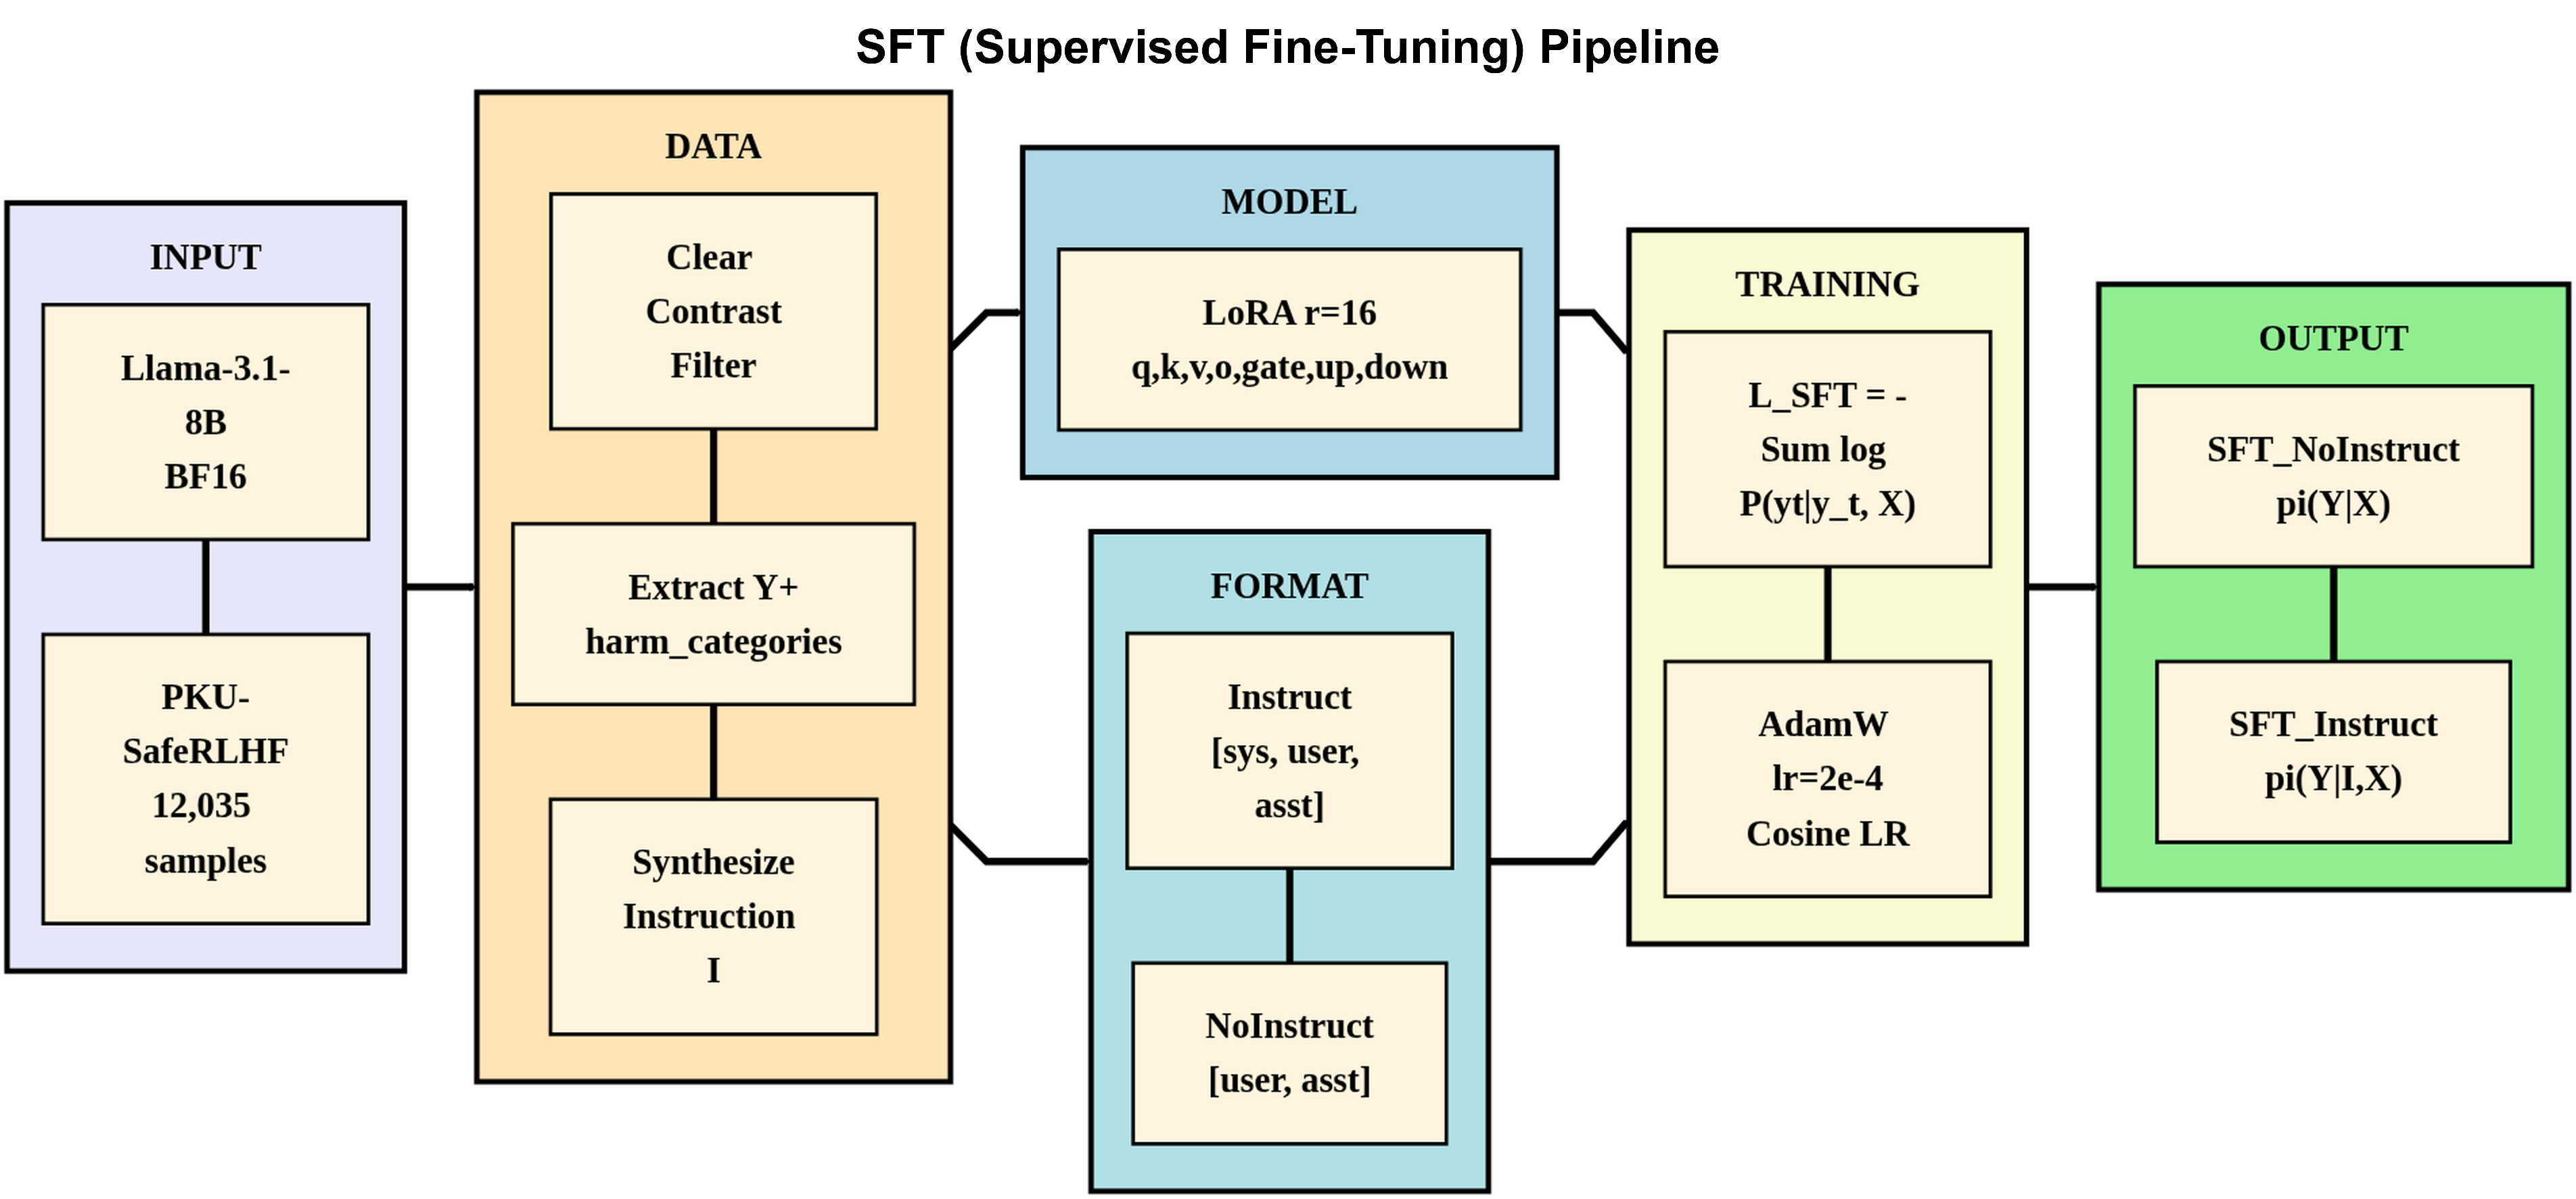
\includegraphics[width=\textwidth]{figures/pipeline/sft_pipeline.pdf}
\caption{\textbf{SFT Training Pipeline.} Starting from Llama-3.1-8B (BF16) and PKU-SafeRLHF dataset (12,035 samples), the pipeline applies clear contrast filtering to extract safe responses ($Y^+$) and harm categories. For the \textbf{Instruct} variant, alignment instructions are synthesized from harm categories and formatted as \texttt{[sys, user, asst]}; for \textbf{NoInstruct}, the format is \texttt{[user, asst]}. LoRA adapters (r=16) target attention and MLP projections. Training uses cross-entropy loss with AdamW optimizer (lr=2e-4) and cosine LR schedule, producing two trained policies: $\pi_{\text{SFT\_NoInstruct}}(Y|X)$ and $\pi_{\text{SFT\_Instruct}}(Y|I,X)$.}
\label{fig:sft_pipeline}
\end{figure}

\paragraph{Overview.} SFT establishes the foundation for all downstream methods by teaching the base Llama-3.1-8B model to generate safe, helpful responses. The training uses TRL's \texttt{SFTTrainer} with standard cross-entropy loss on the safe response tokens only (assistant turns).

\paragraph{Data Preparation.} The PKU-SafeRLHF dataset contains paired responses with safety annotations. We apply \textbf{clear contrast filtering} (\texttt{is\_response\_0\_safe} $\neq$ \texttt{is\_response\_1\_safe}) to ensure unambiguous safety labels, yielding 12,035 training samples. Each sample extracts the safe response ($Y^+$) and associated harm categories (e.g., \texttt{violence}, \texttt{discrimination}).

\paragraph{Instruction Synthesis.} For the Instruct variant, we synthesize alignment instructions from harm categories using a template: \textit{``You are a helpful assistant. The user's query may involve [harm\_categories]. Respond safely and helpfully.''} This conditions the model on explicit safety context during training.

\paragraph{Model Configuration.} We use LoRA~\cite{hu2022lora} with rank $r=16$, $\alpha=16$, targeting attention projections (\texttt{q\_proj, k\_proj, v\_proj, o\_proj}) and MLP layers (\texttt{gate\_proj, up\_proj, down\_proj}). Training uses AdamW optimizer with learning rate $2 \times 10^{-4}$, cosine scheduler, batch size 2, and gradient accumulation 4 (effective batch 8).

% -----------------------------------------------------------------------------
% DPO Pipeline
% -----------------------------------------------------------------------------
\subsection{DPO (Direct Preference Optimization) Pipeline}
\label{sec:appendix_dpo_pipeline}

\begin{figure}[H]
\centering
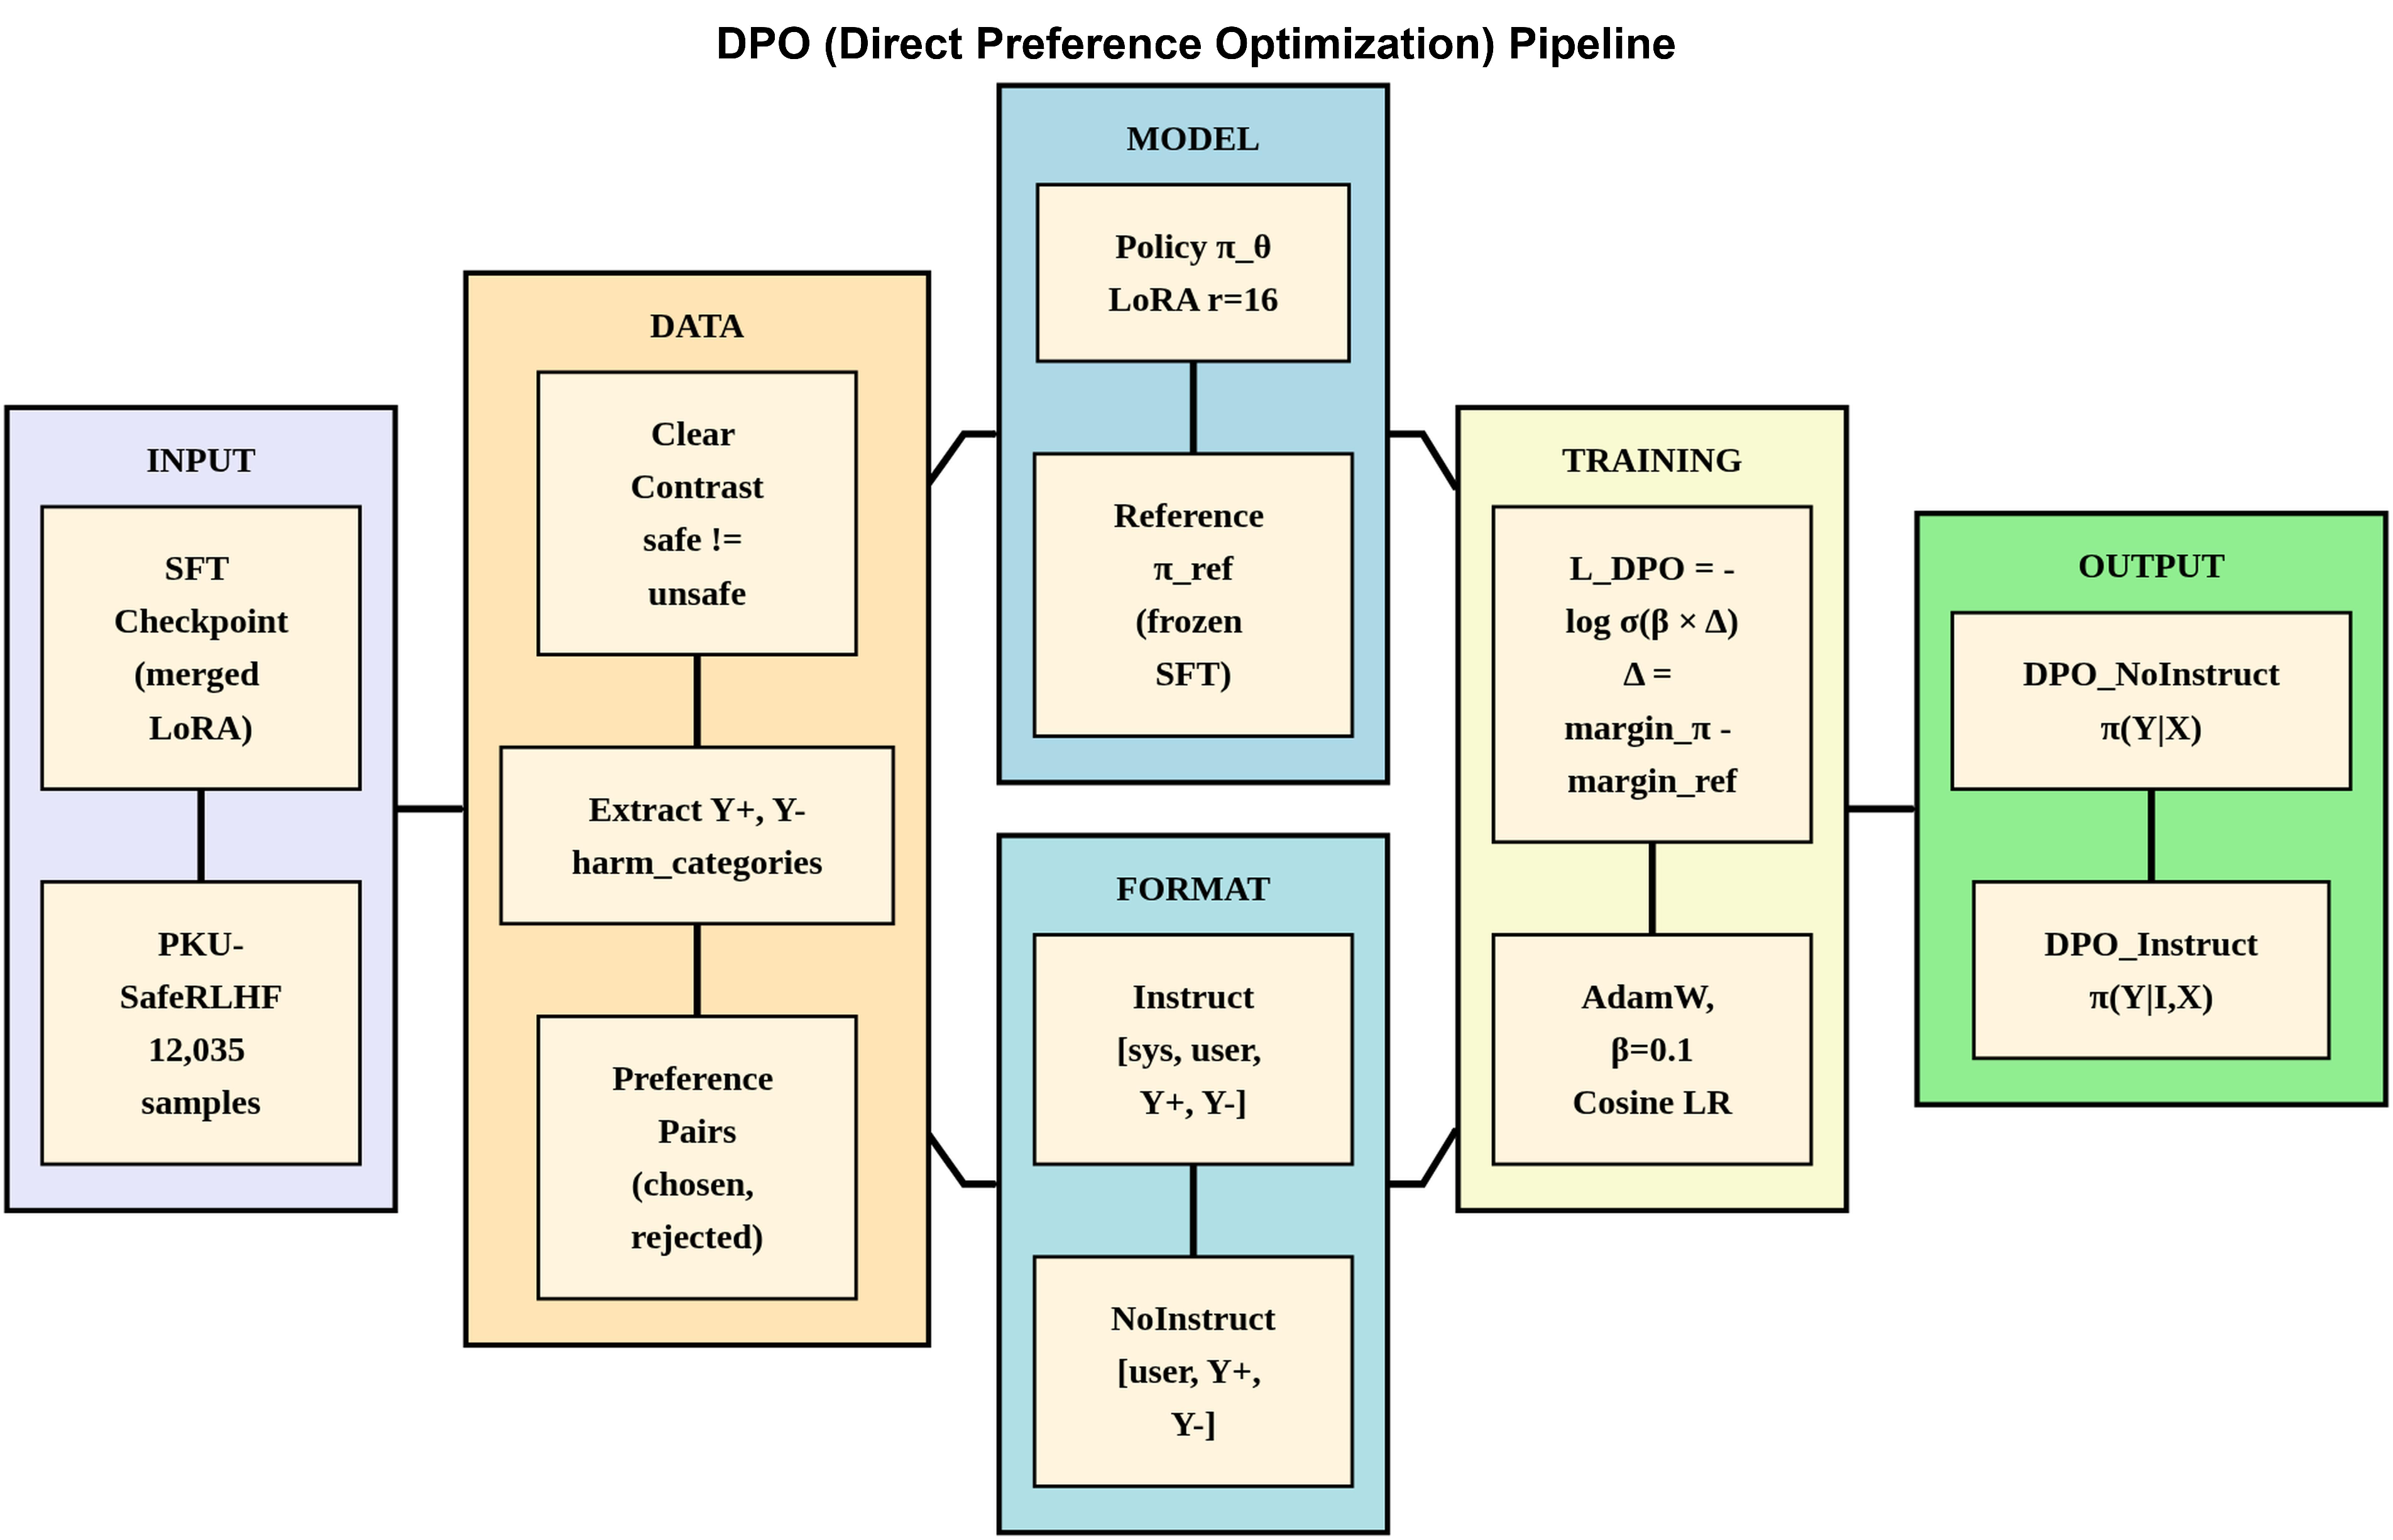
\includegraphics[width=\textwidth]{figures/pipeline/dpo_pipeline.pdf}
\caption{\textbf{DPO Training Pipeline.} Starting from a \textbf{merged SFT checkpoint} (LoRA adapters merged into base weights), the pipeline creates two models: a trainable \textbf{Policy} $\pi_\theta$ with fresh LoRA adapters (r=16) and a \textbf{frozen Reference} $\pi_{\text{ref}}$ (exact copy of merged SFT). PKU-SafeRLHF data undergoes clear contrast filtering (\texttt{is\_response\_0\_safe} $\neq$ \texttt{is\_response\_1\_safe}) to extract preference pairs $(Y^+, Y^-)$ and harm categories. For the \textbf{Instruct} variant, alignment instructions are synthesized from harm categories and formatted as \texttt{[sys, user, chosen, rejected]}; for \textbf{NoInstruct}, the format is \texttt{[user, chosen, rejected]}. Training uses DPO loss: $\mathcal{L}_{\text{DPO}} = -\log \sigma(\beta \cdot \Delta)$ where $\Delta = \text{margin}_\pi - \text{margin}_{\text{ref}}$ and $\beta=0.1$. Output: two trained policies $\pi_{\text{DPO\_NoInstruct}}(Y|X)$ and $\pi_{\text{DPO\_Instruct}}(Y|I,X)$.}
\label{fig:dpo_pipeline}
\end{figure}

\paragraph{Overview.} DPO~\cite{rafailov2023direct} reformulates RLHF as a supervised learning problem on preference pairs, eliminating the need for reward model training. Unlike PPO's online RL loop, DPO directly optimizes the policy using offline preference data.

\paragraph{Model Setup.} DPO requires two models: (1) a trainable \textbf{policy} $\pi_\theta$ initialized from the merged SFT checkpoint with fresh LoRA adapters, and (2) a \textbf{frozen reference} $\pi_{\text{ref}}$ (exact copy of merged SFT). The reference model provides the implicit reward signal through log-probability ratios.

\paragraph{Preference Data.} We extract preference pairs $(Y^+, Y^-)$ from PKU-SafeRLHF where $Y^+$ is the safe response and $Y^-$ is the unsafe response. The same clear contrast filtering ensures unambiguous labels.

\paragraph{Training Configuration.} Training uses TRL's \texttt{DPOTrainer} with $\beta=0.1$ (controls preference strength), learning rate $1 \times 10^{-5}$, batch size 1, and gradient accumulation 8 (effective batch 8). The lower learning rate (vs.\ SFT's $2 \times 10^{-4}$) prevents catastrophic forgetting of SFT capabilities.

% -----------------------------------------------------------------------------
% PPO Pipeline
% -----------------------------------------------------------------------------
\subsection{PPO (Proximal Policy Optimization) Pipeline}
\label{sec:appendix_ppo_pipeline}

\begin{figure}[H]
\centering
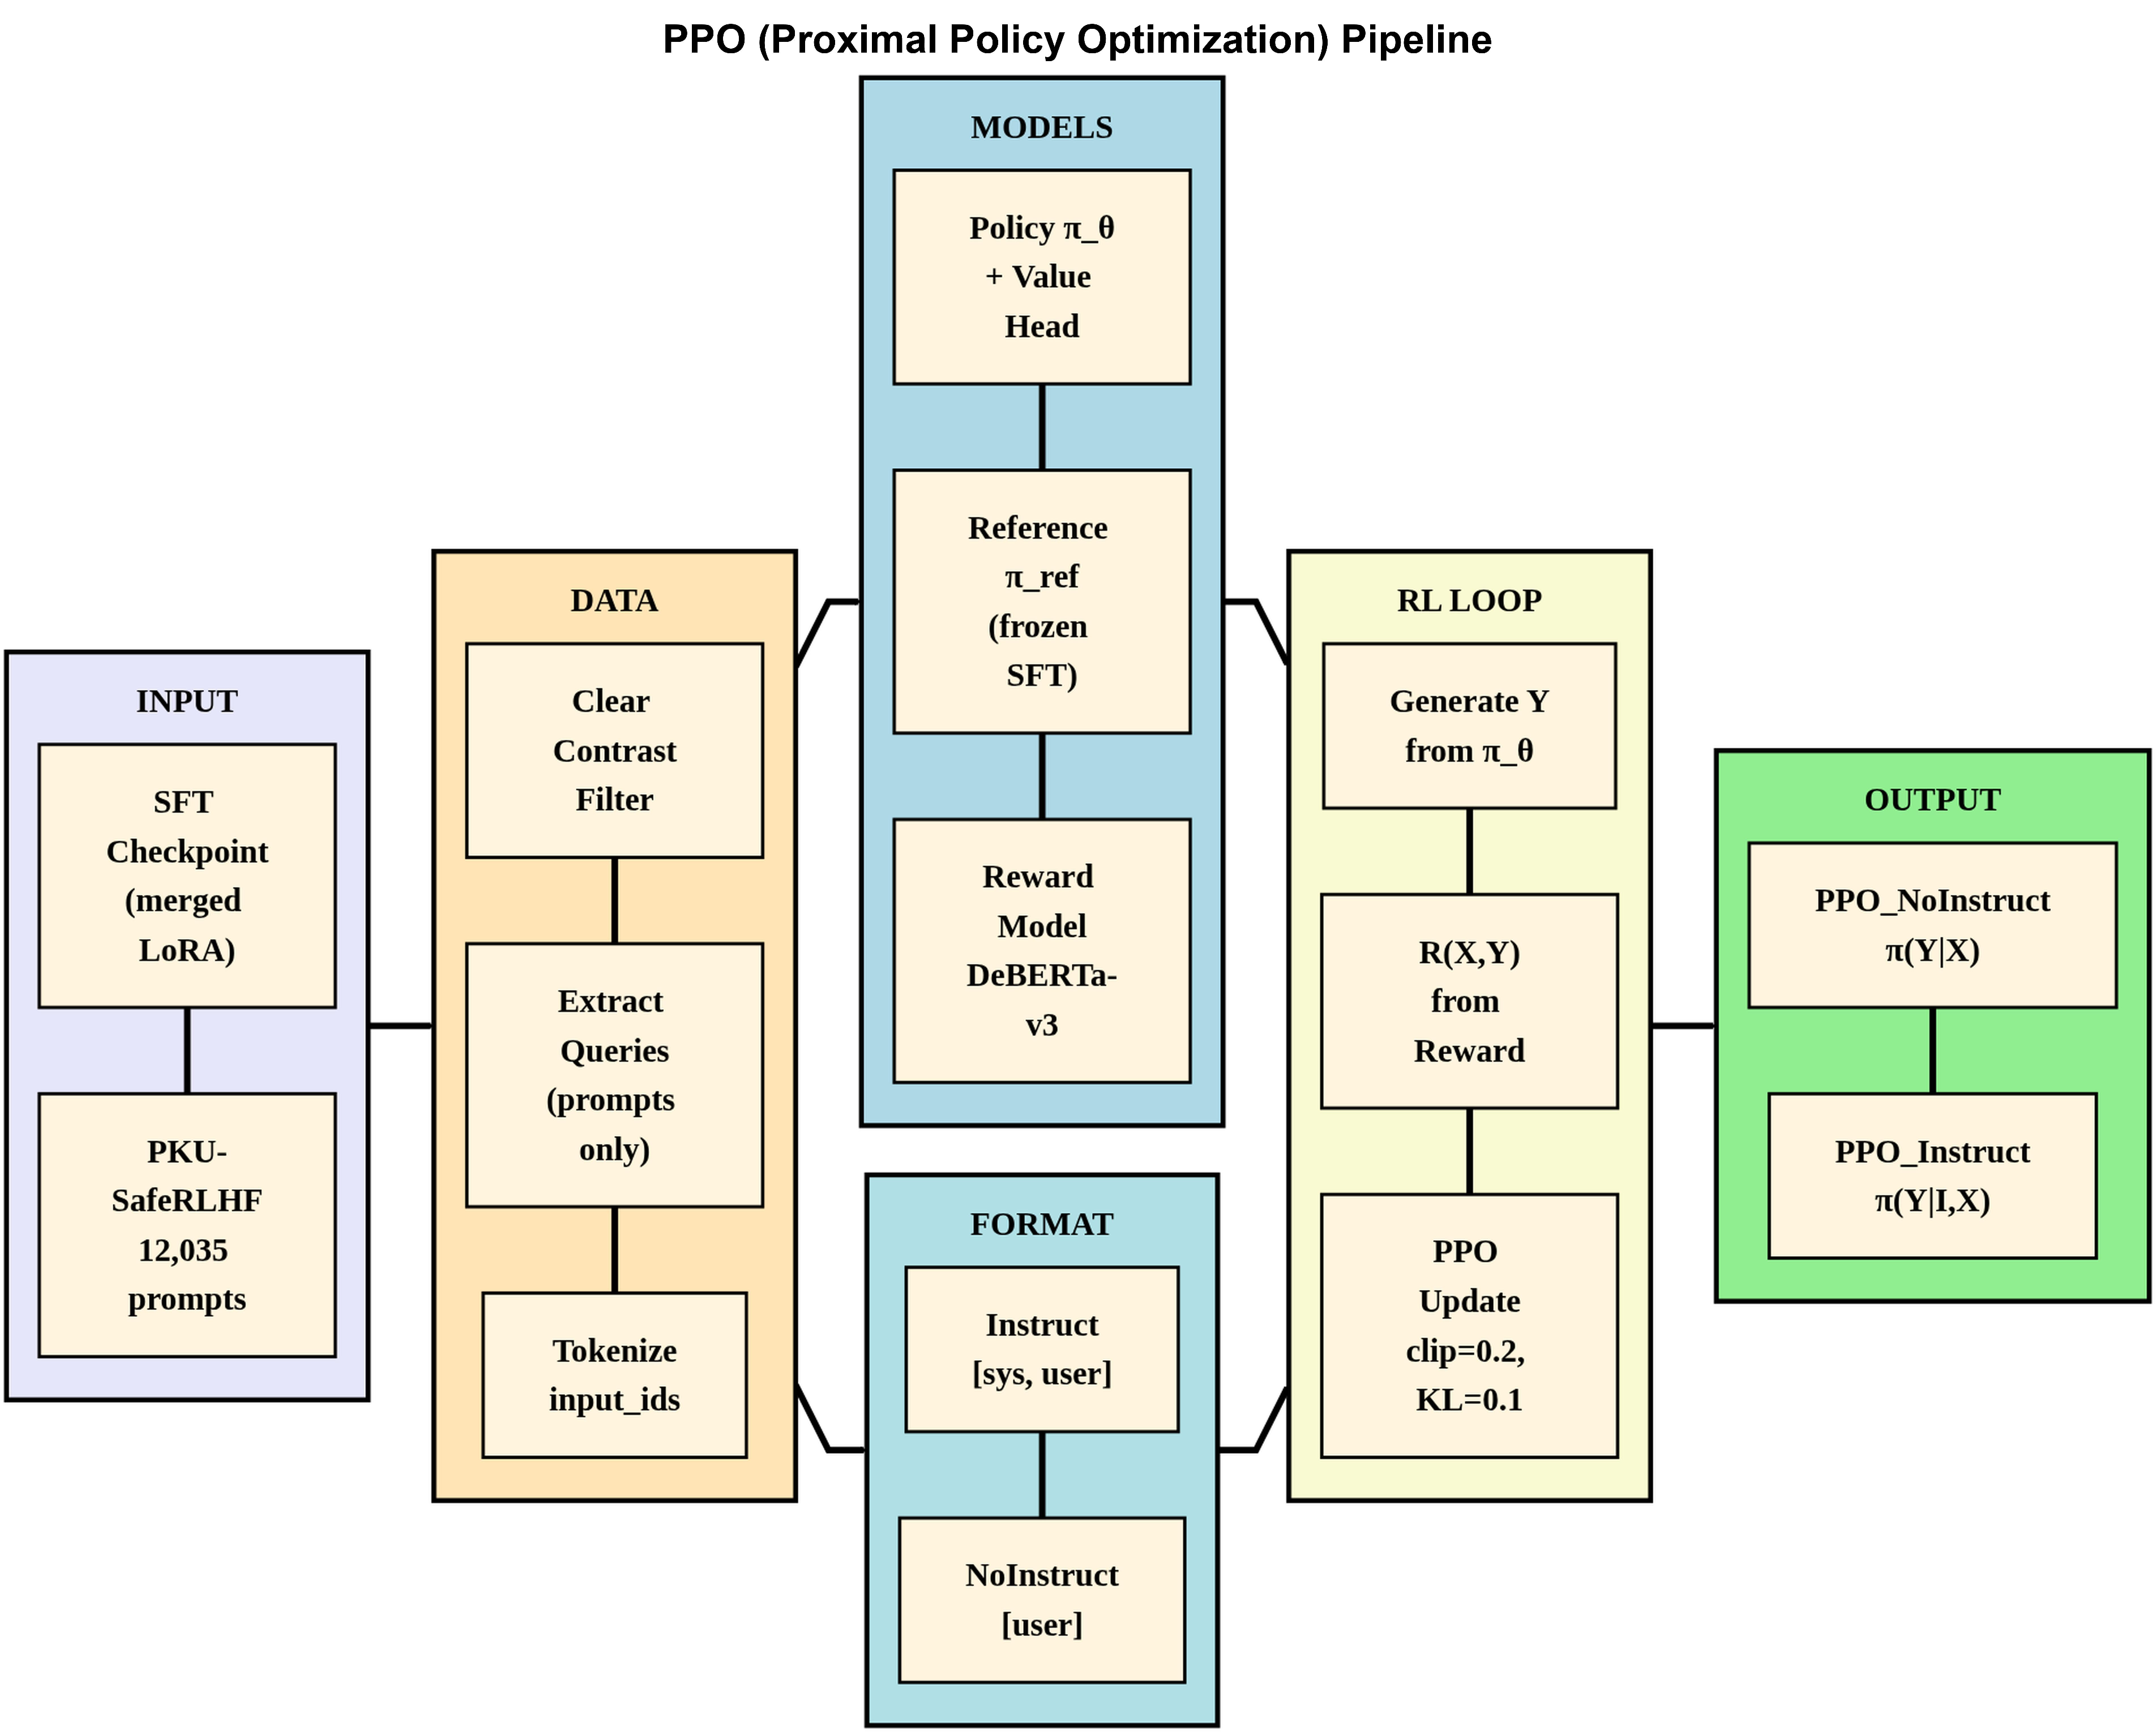
\includegraphics[width=\textwidth]{figures/pipeline/ppo_pipeline.pdf}
\caption{\textbf{PPO Training Pipeline.} Starting from a \textbf{merged SFT checkpoint}, PPO maintains \textbf{three models}: (1) trainable \textbf{Policy} $\pi_\theta$ with a value head for advantage estimation, (2) \textbf{frozen Reference} $\pi_{\text{ref}}$ for KL regularization, and (3) external \textbf{Reward Model} (OpenAssistant DeBERTa-v3-large). Unlike DPO, PPO only requires \textbf{queries} (prompts)---not preference pairs---from PKU-SafeRLHF. The \textbf{online RL loop} iterates: (i) generate responses $Y$ from policy, (ii) score with reward model $R(X,Y)$, (iii) compute GAE advantage ($\gamma=1.0$, $\lambda=0.95$), (iv) PPO update with clipped surrogate objective ($\epsilon=0.2$) and KL penalty (coef$=0.1$). Output: $\pi_{\text{PPO\_NoInstruct}}(Y|X)$ and $\pi_{\text{PPO\_Instruct}}(Y|I,X)$.}
\label{fig:ppo_pipeline}
\end{figure}

\paragraph{Overview.} PPO~\cite{schulman2017proximal} is an \textbf{online reinforcement learning} algorithm that learns from its own generated responses, scored by an external reward model. Unlike DPO's offline approach, PPO iteratively generates, scores, and updates---enabling the model to explore response distributions beyond the static preference dataset.

\paragraph{Three-Model Architecture.} PPO's computational cost stems from maintaining three models simultaneously:

\begin{enumerate}[leftmargin=*]
    \item \textbf{Policy Model} $\pi_\theta$: The trainable language model with an additional \textbf{value head} for advantage estimation. We use TRL's \texttt{AutoModelForCausalLMWithValueHead}, which attaches a linear layer on top of the final hidden states to predict state values $V(s)$. The policy is initialized from the merged SFT checkpoint with LoRA adapters (r=16).

    \item \textbf{Reference Model} $\pi_{\text{ref}}$: A \textbf{frozen copy} of the initial policy (merged SFT). This model never receives gradient updates and serves two purposes: (a) computing KL divergence penalties to prevent reward hacking, and (b) providing the baseline log-probabilities for importance sampling ratios.

    \item \textbf{Reward Model}: We use \texttt{OpenAssistant/reward-model-deberta-v3-large-v2}, an external DeBERTa-v3-large model fine-tuned on human preference data. Given a prompt-response pair $(X, Y)$, it outputs a scalar reward $R(X, Y) \in \mathbb{R}$.
\end{enumerate}

\paragraph{Data Requirements.} Unlike DPO which requires preference pairs $(Y^+, Y^-)$, PPO only needs \textbf{prompts} (queries) from PKU-SafeRLHF. The model generates its own responses during training, which are then scored by the reward model. We apply the same clear contrast filtering to ensure prompt quality.

\paragraph{Online RL Training Loop.} Each PPO training iteration proceeds as follows:

\begin{enumerate}[leftmargin=*]
    \item \textbf{Response Generation}: For a batch of prompts $\{X_i\}$, the policy $\pi_\theta$ generates responses $\{Y_i\}$ using sampling (temperature=0.7, top-k=50). Generation is truncated at 256 new tokens or the EOS token.

    \item \textbf{Reward Scoring}: Each (prompt, response) pair is scored by the reward model: $r_i = R(X_i, Y_i)$. Higher rewards indicate more desirable responses.

    \item \textbf{Advantage Estimation}: We compute advantages using \textbf{Generalized Advantage Estimation (GAE)}~\cite{schulman2015high} with $\gamma=1.0$ (no discounting) and $\lambda=0.95$ (high variance reduction):
    \begin{equation}
        \hat{A}_t = \sum_{l=0}^{\infty} (\gamma \lambda)^l \delta_{t+l}, \quad \text{where} \quad \delta_t = r_t + \gamma V(s_{t+1}) - V(s_t)
    \end{equation}

    \item \textbf{PPO Update}: The policy is updated using the clipped surrogate objective:
    \begin{equation}
        \mathcal{L}^{\text{CLIP}}(\theta) = \mathbb{E}_t \left[ \min\left( \rho_t \hat{A}_t, \text{clip}(\rho_t, 1-\epsilon, 1+\epsilon) \hat{A}_t \right) \right]
    \end{equation}
    where $\rho_t = \frac{\pi_\theta(a_t|s_t)}{\pi_{\text{old}}(a_t|s_t)}$ is the importance sampling ratio and $\epsilon=0.2$ is the clipping threshold.

    \item \textbf{KL Penalty}: An adaptive KL penalty $\beta \cdot D_{\text{KL}}(\pi_\theta \| \pi_{\text{ref}})$ is added to prevent the policy from deviating too far from the reference. We use \texttt{init\_kl\_coef}$=0.1$ and \texttt{target\_kl}$=0.1$---when KL exceeds the target, the coefficient increases; when below, it decreases.
\end{enumerate}

\paragraph{Training Configuration.} We use TRL's \texttt{PPOTrainer} with the following hyperparameters:
\begin{itemize}[leftmargin=*]
    \item Learning rate: $1 \times 10^{-5}$ (same as DPO)
    \item Batch size: 16 prompts per iteration
    \item Mini-batch size: 4 (PPO updates over 4 mini-batches per batch)
    \item Gradient accumulation: 4 steps
    \item PPO epochs: 4 (number of passes over each batch)
    \item Value function coefficient: 0.1 (weight on value loss)
    \item Max gradient norm: 1.0 (gradient clipping)
\end{itemize}

\paragraph{Computational Considerations.} PPO is significantly more expensive than DPO due to: (1) maintaining three models in memory, (2) online generation at each training step, and (3) multiple forward passes for value estimation. For our 8B parameter model with LoRA, PPO training requires approximately 2.5$\times$ the GPU memory of DPO and 3--4$\times$ the wall-clock time per epoch.

\paragraph{Reward Hacking Mitigation.} Without the KL penalty, PPO tends to find degenerate solutions that maximize reward while producing nonsensical text (reward hacking). The adaptive KL penalty and clipped objective together constrain optimization to remain within a ``trust region'' around the initial policy.

% -----------------------------------------------------------------------------
% GRPO Pipeline
% -----------------------------------------------------------------------------
\subsection{GRPO (Group Relative Policy Optimization) Pipeline}
\label{sec:appendix_grpo_pipeline}

\begin{figure}[H]
\centering
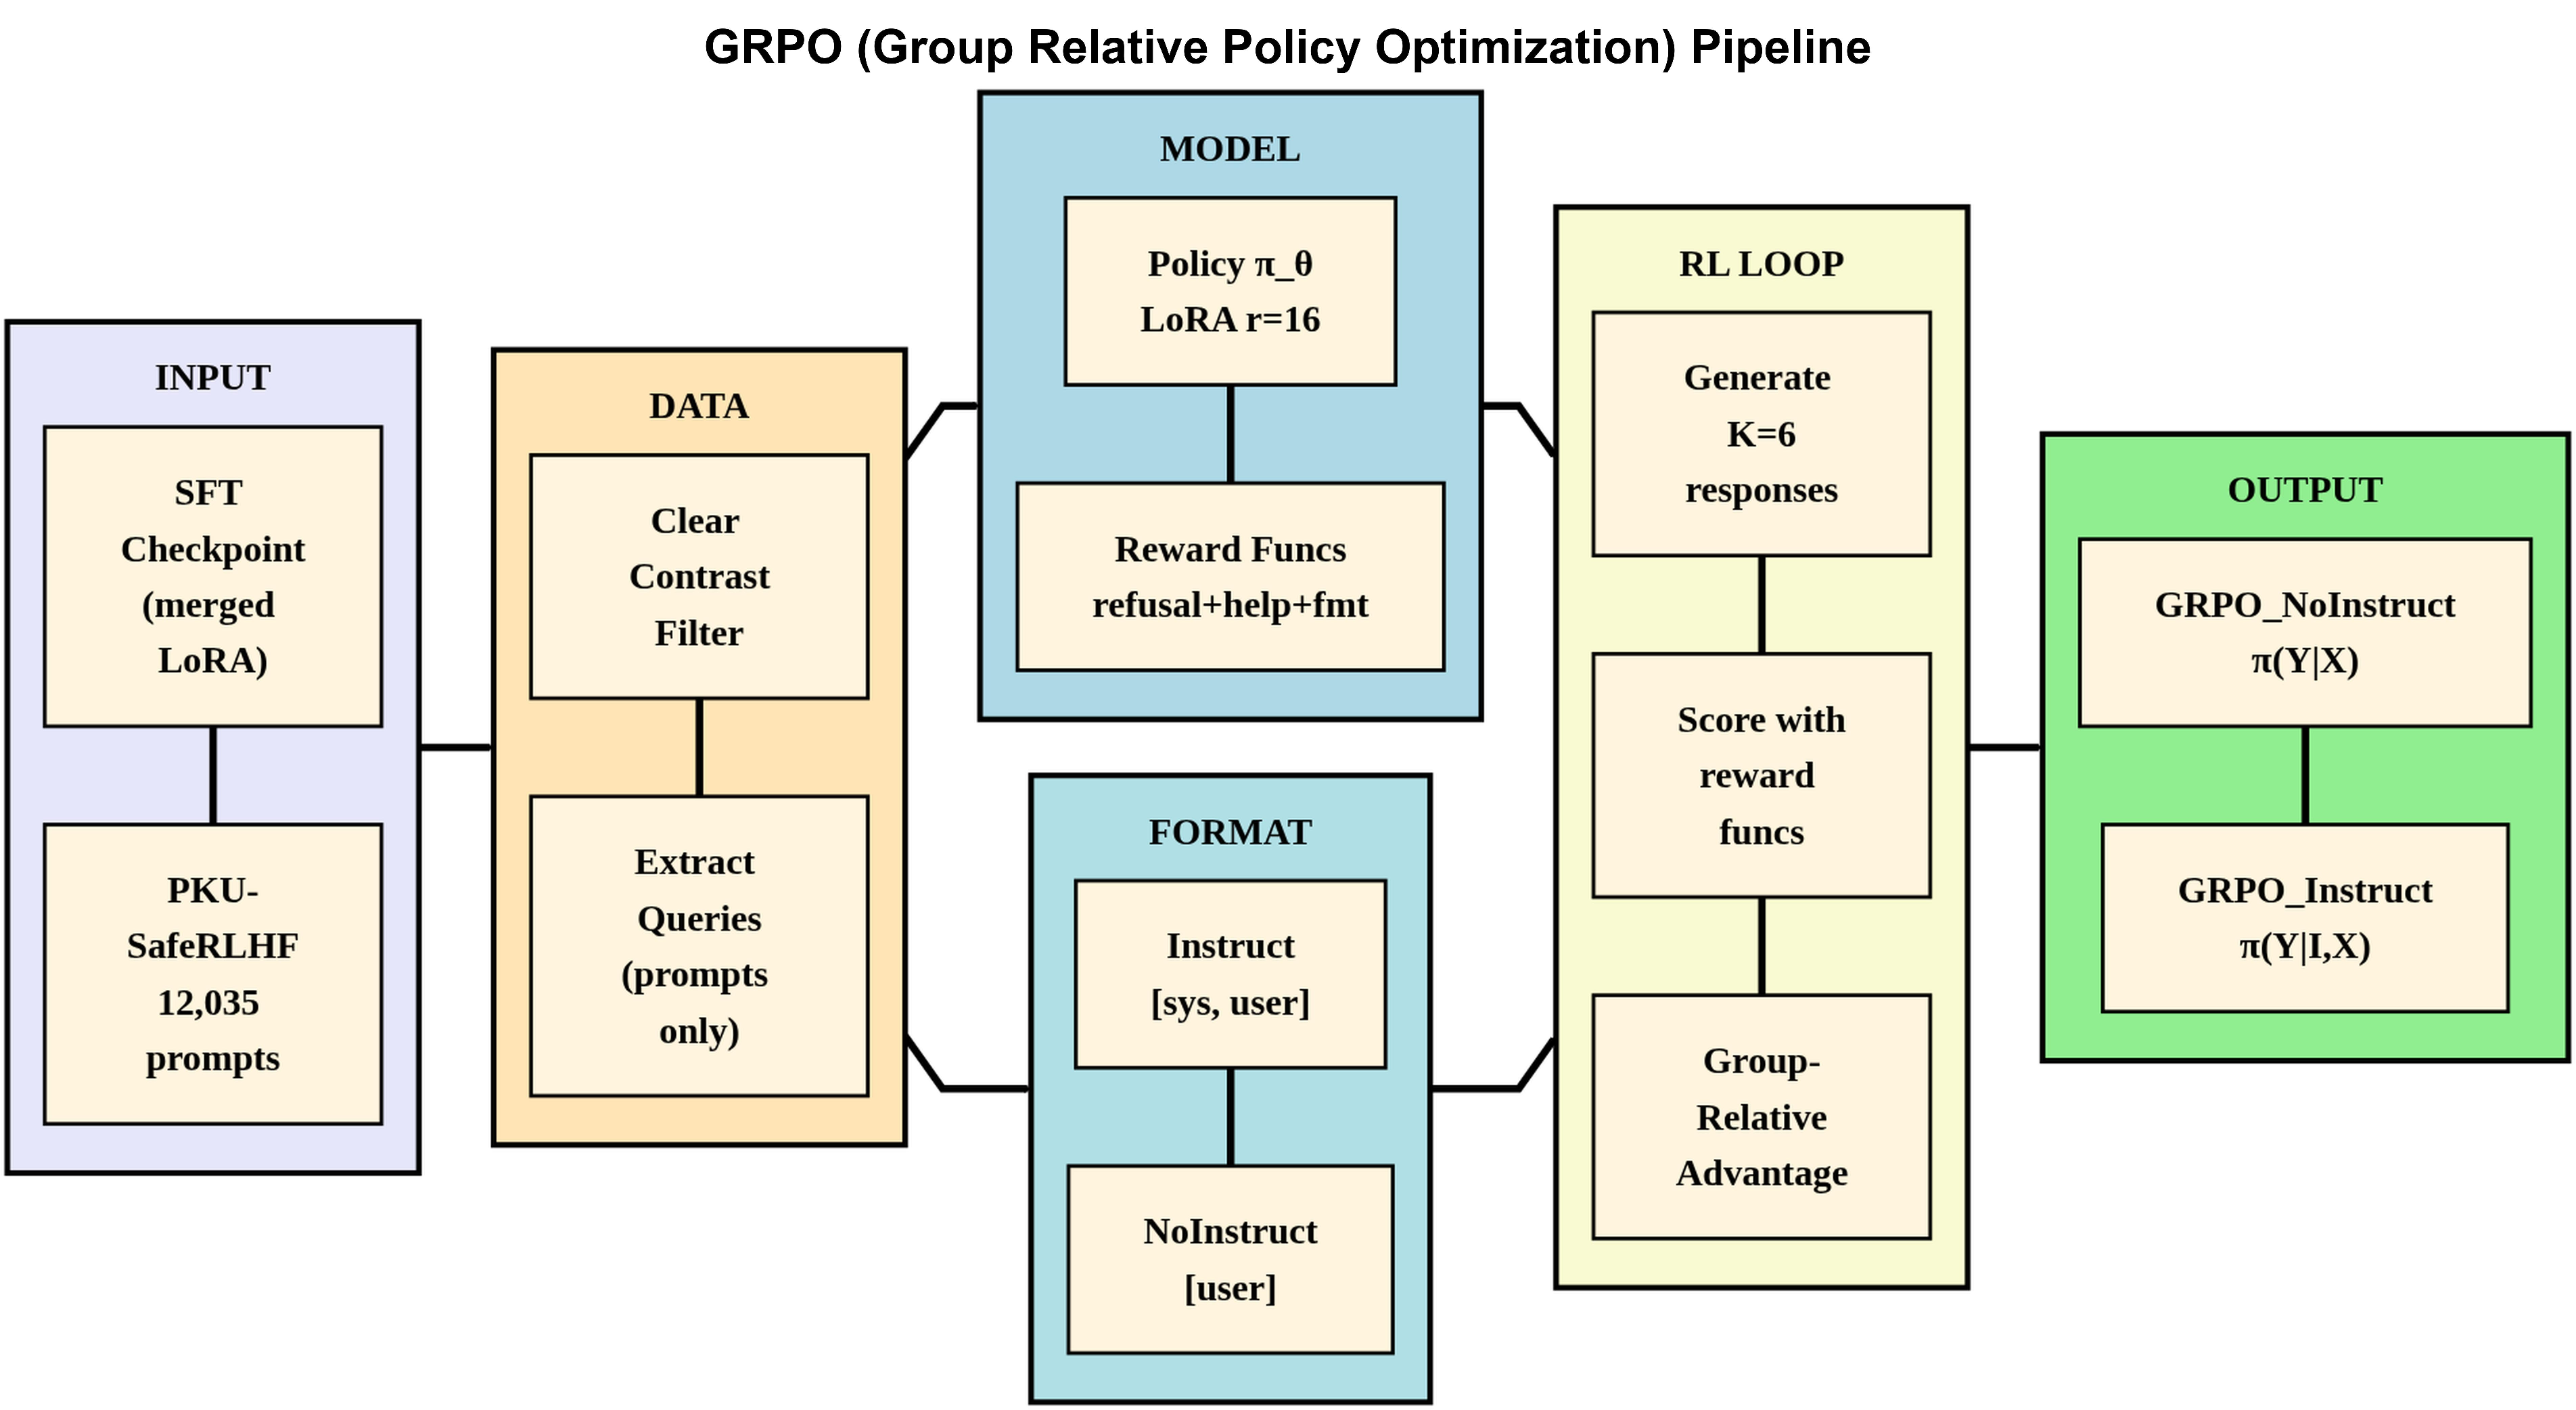
\includegraphics[width=\textwidth]{figures/pipeline/grpo_pipeline.pdf}
\caption{\textbf{GRPO Training Pipeline.} Unlike PPO, GRPO requires \textbf{no reference model}---advantages are computed \textbf{group-relative} within each batch. Starting from a merged SFT checkpoint, the policy $\pi_\theta$ generates $K=6$ responses per prompt. \textbf{Reward functions} (heuristic): (i) \texttt{safety\_refusal} (+1.0 for refusing harmful requests), (ii) \texttt{helpfulness} (+1.0 for substantive responses), (iii) \texttt{format\_quality} (+0.5 for proper structure). The \textbf{group-relative advantage} normalizes rewards within the batch: $\hat{A}(y_i) = (R(y_i) - \mu_{\text{batch}}) / \sigma_{\text{batch}}$, enabling policy gradient updates without KL regularization. Output: $\pi_{\text{GRPO\_NoInstruct}}(Y|X)$ and $\pi_{\text{GRPO\_Instruct}}(Y|I,X)$.}
\label{fig:grpo_pipeline}
\end{figure}

\paragraph{Overview.} GRPO (Group Relative Policy Optimization)~\cite{shao2024deepseekmath} is a recent online RL algorithm that eliminates the need for a \textbf{reference model} by computing advantages \textbf{relative to other responses in the same batch}. This architectural simplification reduces memory requirements while maintaining training stability through group-relative normalization.

\paragraph{Key Innovation: No Reference Model.} Unlike PPO (which requires a frozen reference for KL penalties) and DPO (which requires a reference for implicit reward computation), GRPO computes advantages purely from within-batch statistics:
\begin{equation}
    \hat{A}_{\text{GRPO}}(y_i) = \frac{R(y_i) - \mu_{\text{batch}}}{\sigma_{\text{batch}} + \epsilon}
\end{equation}
where $\mu_{\text{batch}}$ and $\sigma_{\text{batch}}$ are the mean and standard deviation of rewards across all responses in the current batch, and $\epsilon$ is a small constant for numerical stability. This eliminates:
\begin{itemize}[leftmargin=*]
    \item The memory overhead of storing a frozen reference model
    \item The computational cost of reference model forward passes
    \item The hyperparameter sensitivity of KL penalty coefficients
\end{itemize}

\paragraph{Multi-Sample Generation.} For each prompt $X$, GRPO generates \textbf{$K=6$ responses} using sampling (temperature=0.7). This creates a ``group'' of responses that are compared against each other. Responses with above-average rewards receive positive advantages (reinforced), while below-average responses receive negative advantages (suppressed).

\paragraph{Heuristic Reward Functions.} Instead of using a learned reward model (like PPO), we implement three \textbf{heuristic reward functions} tailored for safety alignment:

\begin{enumerate}[leftmargin=*]
    \item \textbf{\texttt{safety\_refusal\_reward}}: Awards $+1.0$ for responses that appropriately refuse harmful requests. Detection uses keyword matching for refusal phrases (``I cannot'', ``I'm not able to'', ``This request is harmful'', etc.) combined with context analysis to avoid false positives.

    \item \textbf{\texttt{helpfulness\_reward}}: Awards $+1.0$ for substantive, informative responses. Penalizes empty or extremely short responses (under 50 characters). Uses simple heuristics: response length, presence of structured content (lists, paragraphs), and absence of filler phrases.

    \item \textbf{\texttt{format\_quality\_reward}}: Awards $+0.5$ for well-structured responses. Checks for proper formatting: complete sentences, appropriate paragraph breaks, and coherent structure. Penalizes responses that end mid-sentence or contain repetitive patterns.
\end{enumerate}

The total reward is the sum: $R(X, Y) = r_{\text{safety}} + r_{\text{help}} + r_{\text{format}}$, ranging from $-0.5$ to $+2.5$.

\paragraph{Why Heuristic Rewards?} Using heuristic rewards instead of a learned reward model offers several advantages:
\begin{itemize}[leftmargin=*]
    \item \textbf{Interpretability}: Each reward component is explicitly defined and debuggable
    \item \textbf{No reward model training}: Eliminates the need for a separate reward model
    \item \textbf{Domain alignment}: Rewards are tailored specifically for safety alignment rather than general preference
    \item \textbf{Computational efficiency}: Simple heuristics are faster than neural network inference
\end{itemize}

However, heuristic rewards have limitations: they may not capture subtle quality differences and can be gamed by the policy if not carefully designed.

\paragraph{Training Loop.} Each GRPO training iteration proceeds as follows:

\begin{enumerate}[leftmargin=*]
    \item \textbf{Prompt Sampling}: Sample a batch of prompts from PKU-SafeRLHF (batch size = 12).

    \item \textbf{Multi-Response Generation}: For each prompt, generate $K=6$ responses using the current policy $\pi_\theta$. This creates 72 total (prompt, response) pairs per batch.

    \item \textbf{Reward Computation}: Score each response using the three heuristic reward functions. Compute combined reward $R(X_i, Y_{i,k})$ for each response.

    \item \textbf{Group-Relative Advantage}: For each prompt's group of $K$ responses, compute normalized advantages:
    \begin{equation}
        \hat{A}_{i,k} = \frac{R(X_i, Y_{i,k}) - \bar{R}_i}{\sigma_{R_i} + \epsilon}
    \end{equation}
    where $\bar{R}_i$ and $\sigma_{R_i}$ are computed over the $K$ responses for prompt $i$.

    \item \textbf{Policy Gradient Update}: Update the policy using REINFORCE-style gradients weighted by advantages:
    \begin{equation}
        \nabla_\theta \mathcal{L} = -\mathbb{E}\left[ \hat{A}_{i,k} \nabla_\theta \log \pi_\theta(Y_{i,k} | X_i) \right]
    \end{equation}
\end{enumerate}

\paragraph{Training Configuration.} We use TRL's \texttt{GRPOTrainer} with the following hyperparameters:
\begin{itemize}[leftmargin=*]
    \item Learning rate: $5 \times 10^{-6}$ (lower than PPO due to higher gradient variance)
    \item Batch size: 12 prompts (72 total responses with $K=6$)
    \item Gradient accumulation: 2 steps
    \item \textbf{Max gradient norm: 0.1} (aggressive clipping---key stability measure)
    \item Number of generations per prompt: $K=6$
    \item LoRA configuration: same as other methods (r=16, $\alpha$=16)
\end{itemize}

\paragraph{Gradient Stability.} GRPO requires \textbf{aggressive gradient clipping} (\texttt{max\_grad\_norm}$=0.1$, vs.\ PPO's $1.0$) because:
\begin{itemize}[leftmargin=*]
    \item Without a reference model's KL penalty, the policy can drift rapidly
    \item Group-relative advantages can have high variance when response quality varies significantly
    \item The REINFORCE estimator inherently has higher variance than PPO's advantage estimator
\end{itemize}

Without aggressive clipping, we observed gradient explosions and training instability after $\sim$500 steps.

\paragraph{Comparison with PPO.}
\begin{center}
\begin{tabular}{lcc}
\toprule
\textbf{Aspect} & \textbf{PPO} & \textbf{GRPO} \\
\midrule
Reference model & Required (frozen) & Not required \\
Reward model & Neural network & Heuristic functions \\
Advantage computation & GAE with value head & Group-relative normalization \\
KL regularization & Adaptive penalty & None (relies on grad clipping) \\
Memory overhead & High (3 models) & Low (1 model) \\
Generations per prompt & 1 & $K=6$ \\
\bottomrule
\end{tabular}
\end{center}

% -----------------------------------------------------------------------------
% CITA Pipeline
% -----------------------------------------------------------------------------
\subsection{CITA (Contrastive Instruction-Tuned Alignment) Pipeline}
\label{sec:appendix_cita_pipeline}

\begin{figure}[H]
\centering
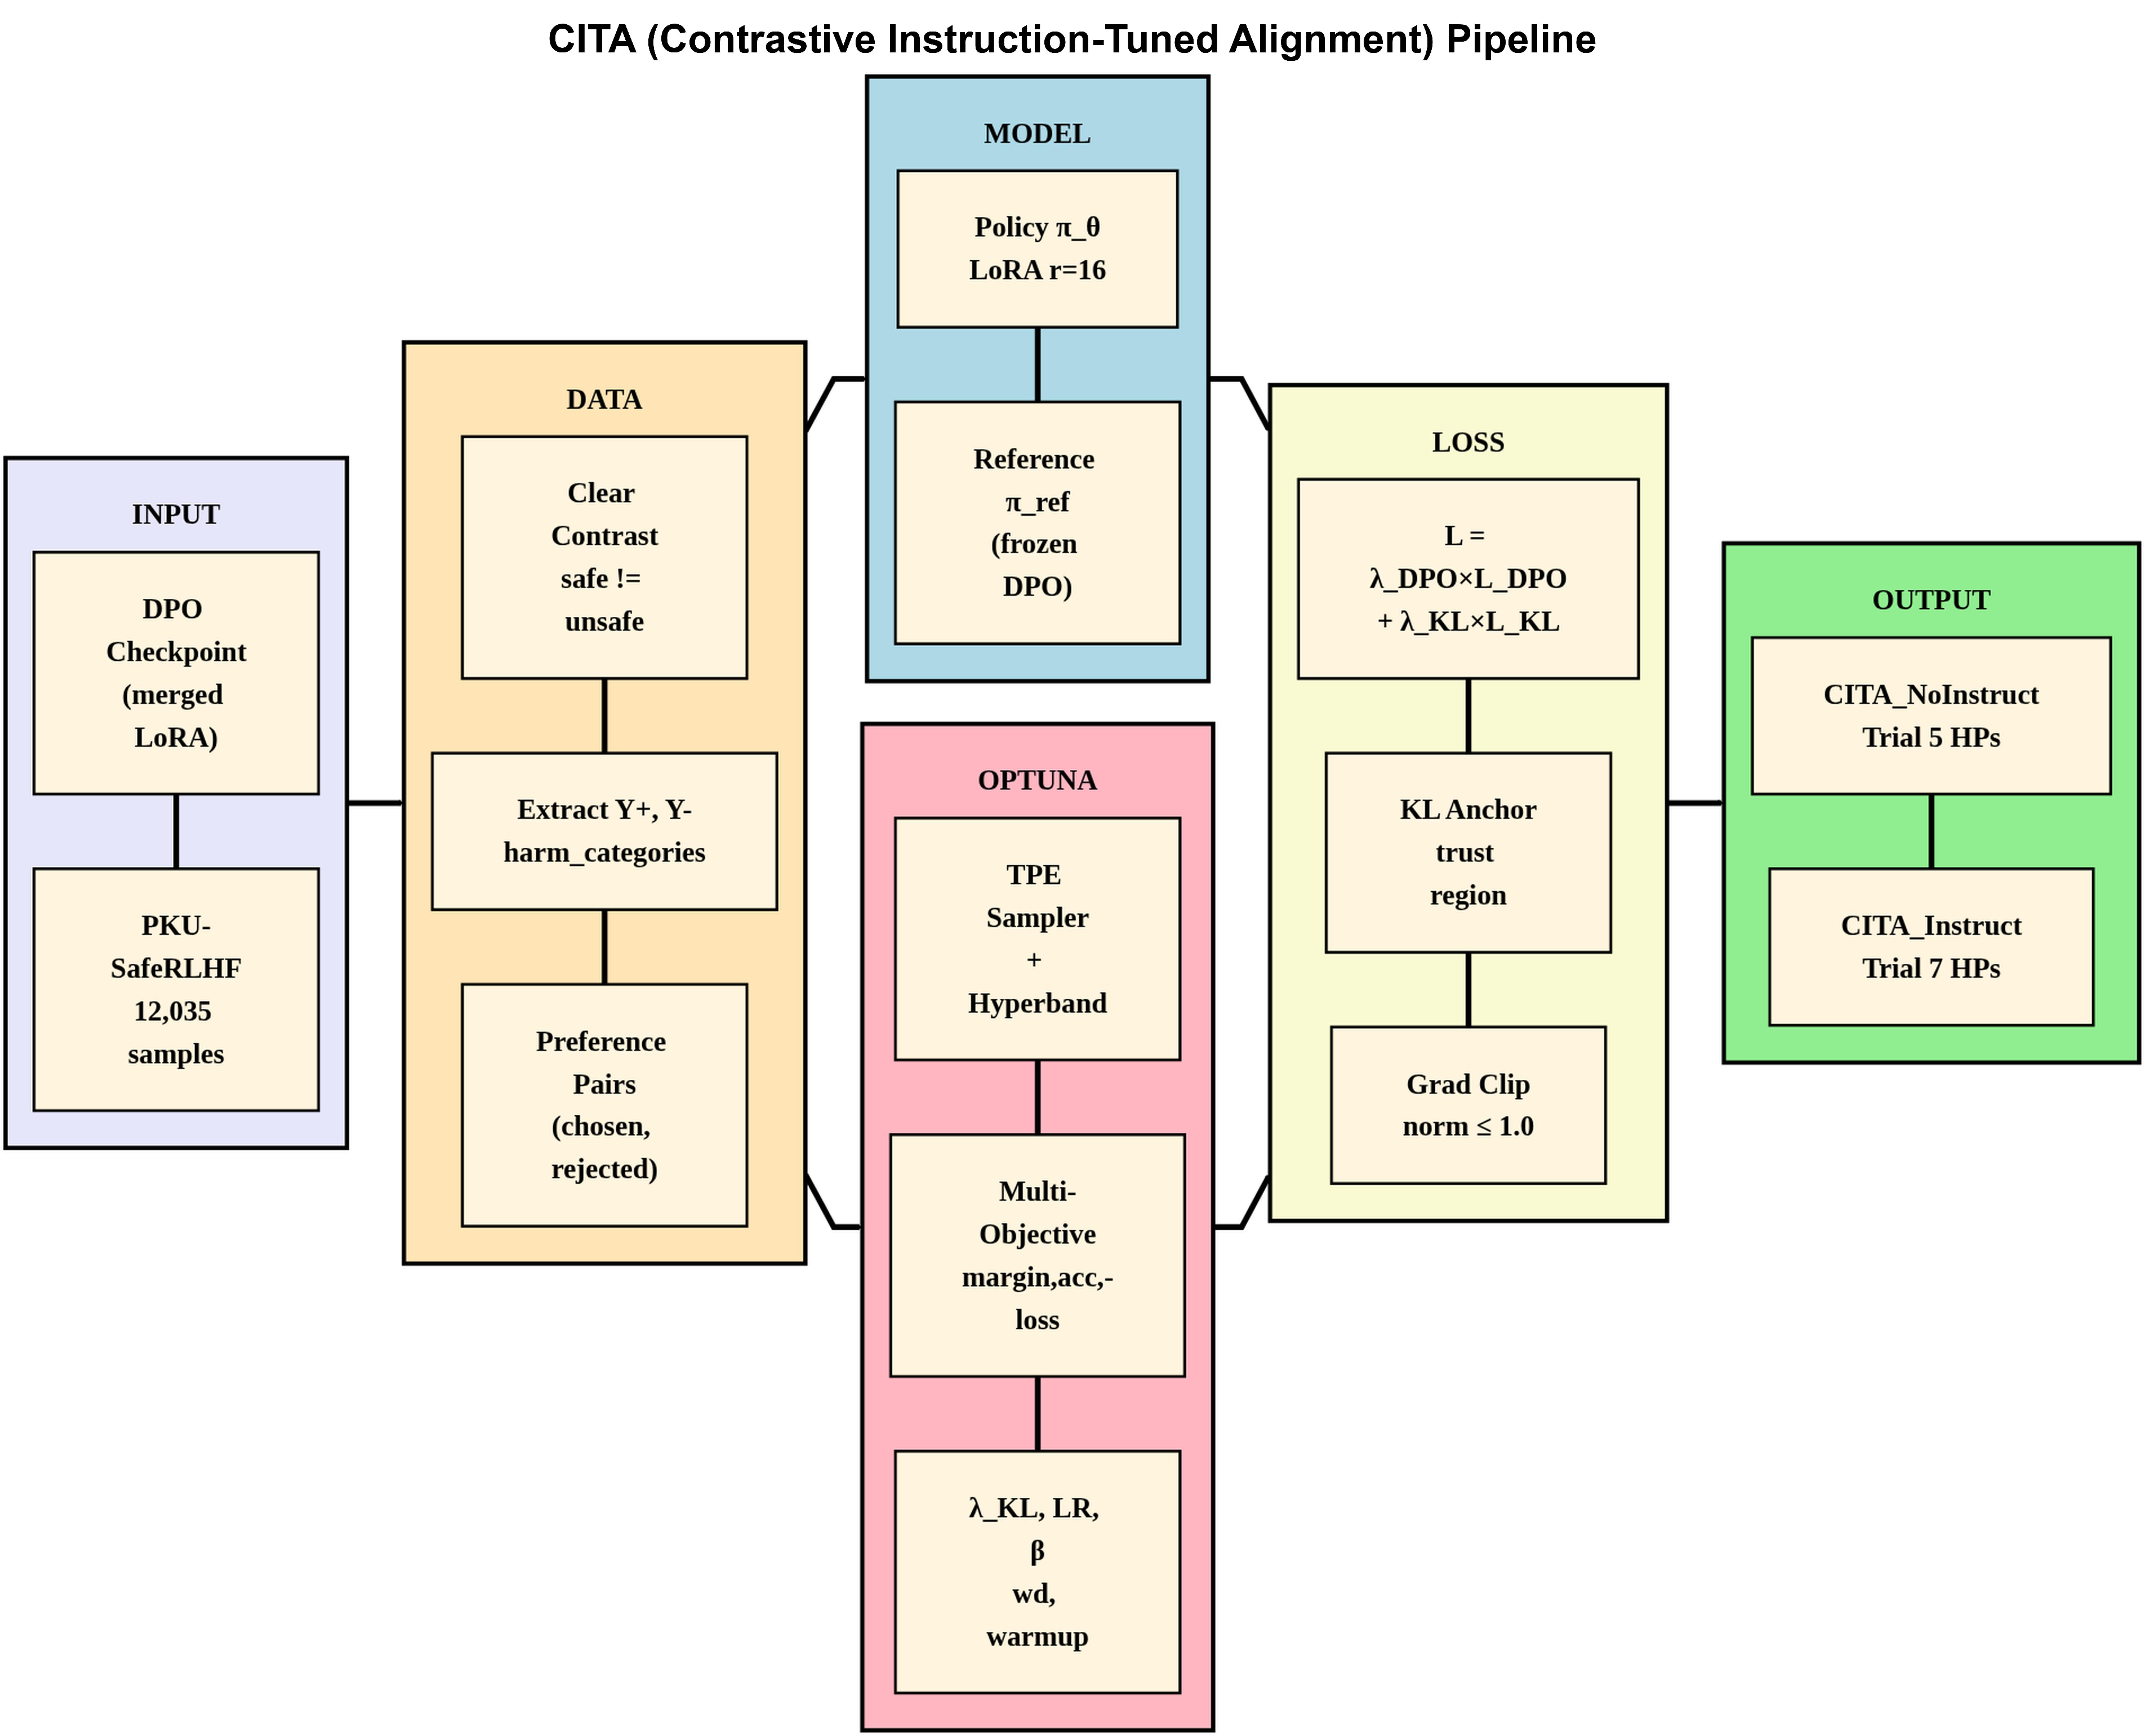
\includegraphics[width=\textwidth]{figures/pipeline/cita_pipeline.pdf}
\caption{\textbf{CITA Training Pipeline.} CITA \textbf{stacks on DPO} (not SFT) and adds a \textbf{mandatory KL anchor} for stable multi-regime switching. \textbf{Unified loss}: $\mathcal{L}_{\text{CITA}} = \lambda_{\text{DPO}} \cdot \mathcal{L}_{\text{DPO}} + \lambda_{\text{KL}} \cdot \mathcal{L}_{\text{KL}}$, where $\mathcal{L}_{\text{KL}} = \frac{1}{2}[\text{mean}(\log \pi_\theta - \log \pi_{\text{ref}})_{\text{chosen}} + \text{mean}(\log \pi_\theta - \log \pi_{\text{ref}})_{\text{rejected}}]$. \textbf{NO $\mathcal{L}_{\text{SFT}}$}---adding SFT loss causes catastrophic interference on DPO-tuned models (margin collapse $2.95 \rightarrow 0.10$). \textbf{Hyperparameter tuning}: Optuna TPE sampler with Hyperband pruner optimizes $(\lambda_{\text{KL}}, \text{LR}, \beta, \text{weight\_decay}, \text{warmup\_ratio})$ via multi-objective optimization (maximize margin, accuracy; minimize eval\_loss). \textbf{Instruct} variant uses $\sim$50\% lower LR due to longer sequences (30--40\% more tokens). Final models use \textbf{Trial 5} HPs (NoInstruct: margin$=$6.95) and \textbf{Trial 7} HPs (Instruct: margin$=$7.52). Gradient clipping ($\|\nabla\| \leq 1.0$) prevents training explosion. Output: $\pi_{\text{CITA\_NoInstruct}}(Y|X)$ and $\pi_{\text{CITA\_Instruct}}(Y|I,X)$.}
\label{fig:cita_pipeline}
\end{figure}

\paragraph{Overview.} CITA (Contrastive Instruction-Tuned Alignment) is our proposed method that \textbf{stacks on a DPO-trained model} rather than SFT, adding a carefully designed KL anchor term for stable multi-regime instruction following. The key insight is that DPO already establishes strong preference alignment; CITA refines this with instruction-conditioned behavior while preventing catastrophic forgetting.

\paragraph{Why Stack on DPO (Not SFT)?} DPO training produces a model that has learned to distinguish between preferred and dispreferred responses. Starting from this checkpoint preserves:
\begin{itemize}[leftmargin=*]
    \item The implicit reward model embedded in log-probability ratios
    \item Preference-aligned response distributions
    \item Safety-aware generation patterns from DPO's preference optimization
\end{itemize}

Starting from SFT would discard these learned preferences, requiring CITA to relearn both preference alignment and instruction conditioning simultaneously.

\paragraph{The Unified Loss Function.} CITA uses a custom \texttt{CITATrainer} (inheriting from TRL's \texttt{DPOTrainer}) with a unified loss:
\begin{equation}
    \mathcal{L}_{\text{CITA}} = \lambda_{\text{DPO}} \cdot \mathcal{L}_{\text{DPO}} + \lambda_{\text{KL}} \cdot \mathcal{L}_{\text{KL}}
\end{equation}
where:
\begin{itemize}[leftmargin=*]
    \item $\mathcal{L}_{\text{DPO}}$: The standard DPO loss (identical to~\cite{rafailov2023direct}), providing continued preference learning. We reuse TRL's \texttt{DPOTrainer.dpo\_loss()} for apple-to-apple comparison with baseline DPO.

    \item $\mathcal{L}_{\text{KL}}$: A \textbf{KL anchor term} that prevents the policy from drifting too far from the reference (frozen DPO checkpoint):
    \begin{equation}
        \mathcal{L}_{\text{KL}} = \frac{1}{2} \left[ \text{mean}\left(\log \pi_\theta(Y^+ | X) - \log \pi_{\text{ref}}(Y^+ | X)\right) + \text{mean}\left(\log \pi_\theta(Y^- | X) - \log \pi_{\text{ref}}(Y^- | X)\right) \right]
    \end{equation}
    This is computed over \textbf{both chosen and rejected} responses, ensuring the policy stays close to the reference distribution across the entire response space.

    \item $\lambda_{\text{DPO}} = 1.0$ (fixed) and $\lambda_{\text{KL}} \in [0.0001, 0.01]$ (tuned via Optuna).
\end{itemize}

\paragraph{Critical Design Decision: NO $\mathcal{L}_{\text{SFT}}$.} Early experiments included an SFT loss term ($\lambda_{\text{SFT}} \cdot \mathcal{L}_{\text{SFT}}$) to encourage fluent generation on chosen responses. However, this caused \textbf{catastrophic interference}:
\begin{itemize}[leftmargin=*]
    \item DPO margin collapsed from $2.95 \rightarrow 0.10$ (near-random preference)
    \item Accuracy dropped from $83\% \rightarrow 51\%$ (coin-flip performance)
    \item The SFT loss encouraged high probability on chosen responses regardless of the rejected response, destroying the contrastive signal
\end{itemize}

The unified loss ($\mathcal{L}_{\text{DPO}} + \lambda_{\text{KL}} \cdot \mathcal{L}_{\text{KL}}$) preserves the contrastive preference signal while adding instruction-conditioning through the data formatting (Instruct variant includes system prompts with harm categories).

\paragraph{Hyperparameter Search with Optuna.} CITA's performance is sensitive to hyperparameters, motivating automated tuning via Optuna~\cite{akiba2019optuna}:

\textbf{Search Space:}
\begin{itemize}[leftmargin=*]
    \item $\lambda_{\text{KL}} \in [0.0001, 0.01]$ (log-uniform)
    \item Learning rate $\in [1 \times 10^{-6}, 2 \times 10^{-5}]$ (log-uniform)
    \item $\beta \in [0.05, 0.3]$ (DPO temperature)
    \item Weight decay $\in [0.001, 0.1]$ (log-uniform)
    \item Warmup ratio $\in [0.03, 0.15]$ (uniform)
\end{itemize}

\textbf{Multi-Objective Optimization:} We optimize three objectives simultaneously:
\begin{enumerate}[leftmargin=*]
    \item \textbf{Maximize margin}: $\text{chosen\_reward} - \text{rejected\_reward}$ (higher = better preference discrimination)
    \item \textbf{Maximize accuracy}: Fraction of samples where $\text{chosen\_reward} > \text{rejected\_reward}$
    \item \textbf{Minimize eval\_loss}: Validation loss on held-out preference pairs
\end{enumerate}

\textbf{Search Algorithm:}
\begin{itemize}[leftmargin=*]
    \item \textbf{TPE Sampler} (Tree-structured Parzen Estimator): Bayesian optimization that models $P(\text{good} | \text{hyperparameters})$ using density estimation. More sample-efficient than random/grid search.
    \item \textbf{Hyperband Pruner}: Early-stopping strategy that terminates poorly-performing trials after few training steps. Uses successive halving to allocate more resources to promising configurations.
    \item Total trials: 15 (NoInstruct) + 15 (Instruct)
    \item Early stopping: Prune if margin $< 0.5$ after 100 steps (gradient explosion detection: \texttt{grad\_norm} $> 50$ triggers immediate pruning)
\end{itemize}

\paragraph{Conditional Hyperparameter Space.} The Instruct variant uses \textbf{50\% lower learning rates} than NoInstruct because:
\begin{itemize}[leftmargin=*]
    \item System prompts add 30--40\% more tokens per sample
    \item Longer sequences produce larger gradient magnitudes
    \item Lower LR compensates to maintain stable training
\end{itemize}

This is implemented as a conditional search space in Optuna: if \texttt{variant == "Instruct"}, the LR upper bound is halved.

\paragraph{Selected Hyperparameters.} After Optuna search, the best configurations were:

\textbf{Trial 5 (NoInstruct):}
\begin{itemize}[leftmargin=*]
    \item $\lambda_{\text{KL}} = 0.000520$
    \item Learning rate $= 6.83 \times 10^{-6}$
    \item $\beta = 0.1191$
    \item Weight decay $= 0.0047$
    \item Warmup ratio $= 0.086$
    \item \textbf{Final margin: 6.95}
\end{itemize}

\textbf{Trial 7 (Instruct):}
\begin{itemize}[leftmargin=*]
    \item $\lambda_{\text{KL}} = 0.000235$
    \item Learning rate $= 5.41 \times 10^{-6}$
    \item $\beta = 0.1067$
    \item Weight decay $= 0.0127$
    \item Warmup ratio $= 0.054$
    \item \textbf{Final margin: 7.52}
\end{itemize}

Note that the Instruct variant achieves \textbf{higher margin} despite using lower LR, suggesting that explicit instruction conditioning provides a stronger learning signal.

\paragraph{Gradient Explosion Detection.} The \texttt{CITATrainer} includes custom gradient monitoring in \texttt{training\_step()}:
\begin{itemize}[leftmargin=*]
    \item After each backward pass, compute \texttt{total\_norm} across all parameters
    \item If \texttt{total\_norm} $> 50$: log warning and trigger Optuna's \texttt{TrialPruned} exception
    \item Standard gradient clipping (\texttt{max\_grad\_norm}$=1.0$) is applied after explosion check
\end{itemize}

This prevents wasted compute on diverging trials and provides diagnostic information for hyperparameter debugging.

\paragraph{Training Configuration.} Final training uses the selected Optuna HPs with:
\begin{itemize}[leftmargin=*]
    \item Batch size: 1 (due to long sequences with system prompts)
    \item Gradient accumulation: 8 steps (effective batch 8)
    \item Max sequence length: 2048 tokens
    \item LoRA: r=16, $\alpha$=16, targeting all attention + MLP projections
    \item Optimizer: AdamW with cosine LR schedule
    \item Training epochs: 1 (single pass over PKU-SafeRLHF)
\end{itemize}

\paragraph{CITATrainer Implementation Details.} The custom trainer overrides three key methods:

\begin{enumerate}[leftmargin=*]
    \item \texttt{compute\_loss()}: Computes unified loss $\mathcal{L}_{\text{CITA}}$ by calling parent's \texttt{dpo\_loss()} and adding the KL anchor term.

    \item \texttt{training\_step()}: Adds gradient explosion detection after backward pass, before optimizer step.

    \item \texttt{log()}: Extended logging for margin, accuracy, KL divergence, and gradient norm at each step for Optuna objective tracking.
\end{enumerate}

The trainer inherits all other functionality (data loading, evaluation, checkpointing) from TRL's \texttt{DPOTrainer}, ensuring consistency with baseline DPO.

\paragraph{Comparison with DPO.}
\begin{center}
\begin{tabular}{lcc}
\toprule
\textbf{Aspect} & \textbf{DPO} & \textbf{CITA} \\
\midrule
Starting checkpoint & Merged SFT & Merged DPO \\
Loss function & $\mathcal{L}_{\text{DPO}}$ only & $\mathcal{L}_{\text{DPO}} + \lambda_{\text{KL}} \mathcal{L}_{\text{KL}}$ \\
KL regularization & Implicit (via $\pi_{\text{ref}}$ in loss) & Explicit anchor term \\
Hyperparameter tuning & Manual & Optuna (TPE + Hyperband) \\
Instruction conditioning & Via data format only & Data format + explicit KL constraint \\
Typical margin & 2.5--3.5 & 6.5--7.5 \\
\bottomrule
\end{tabular}
\end{center}

% =============================================================================
% EVALUATION PIPELINE (Unified for all 5 benchmarks)
% =============================================================================
\newpage
\section{Evaluation Pipeline}
\label{sec:appendix_evaluation_pipeline}

This section describes the \textbf{unified evaluation pipeline} used to assess instruction-conditioned behavioral switching across all five benchmarks (Table~\ref{tab:benchmarks} in the main text). Unlike the training pipelines---which differ fundamentally in architecture (3-model PPO, no-reference GRPO, stacked CITA)---all evaluation benchmarks share a \textbf{common evaluation methodology} with benchmark-specific metrics.

\begin{figure}[H]
\centering
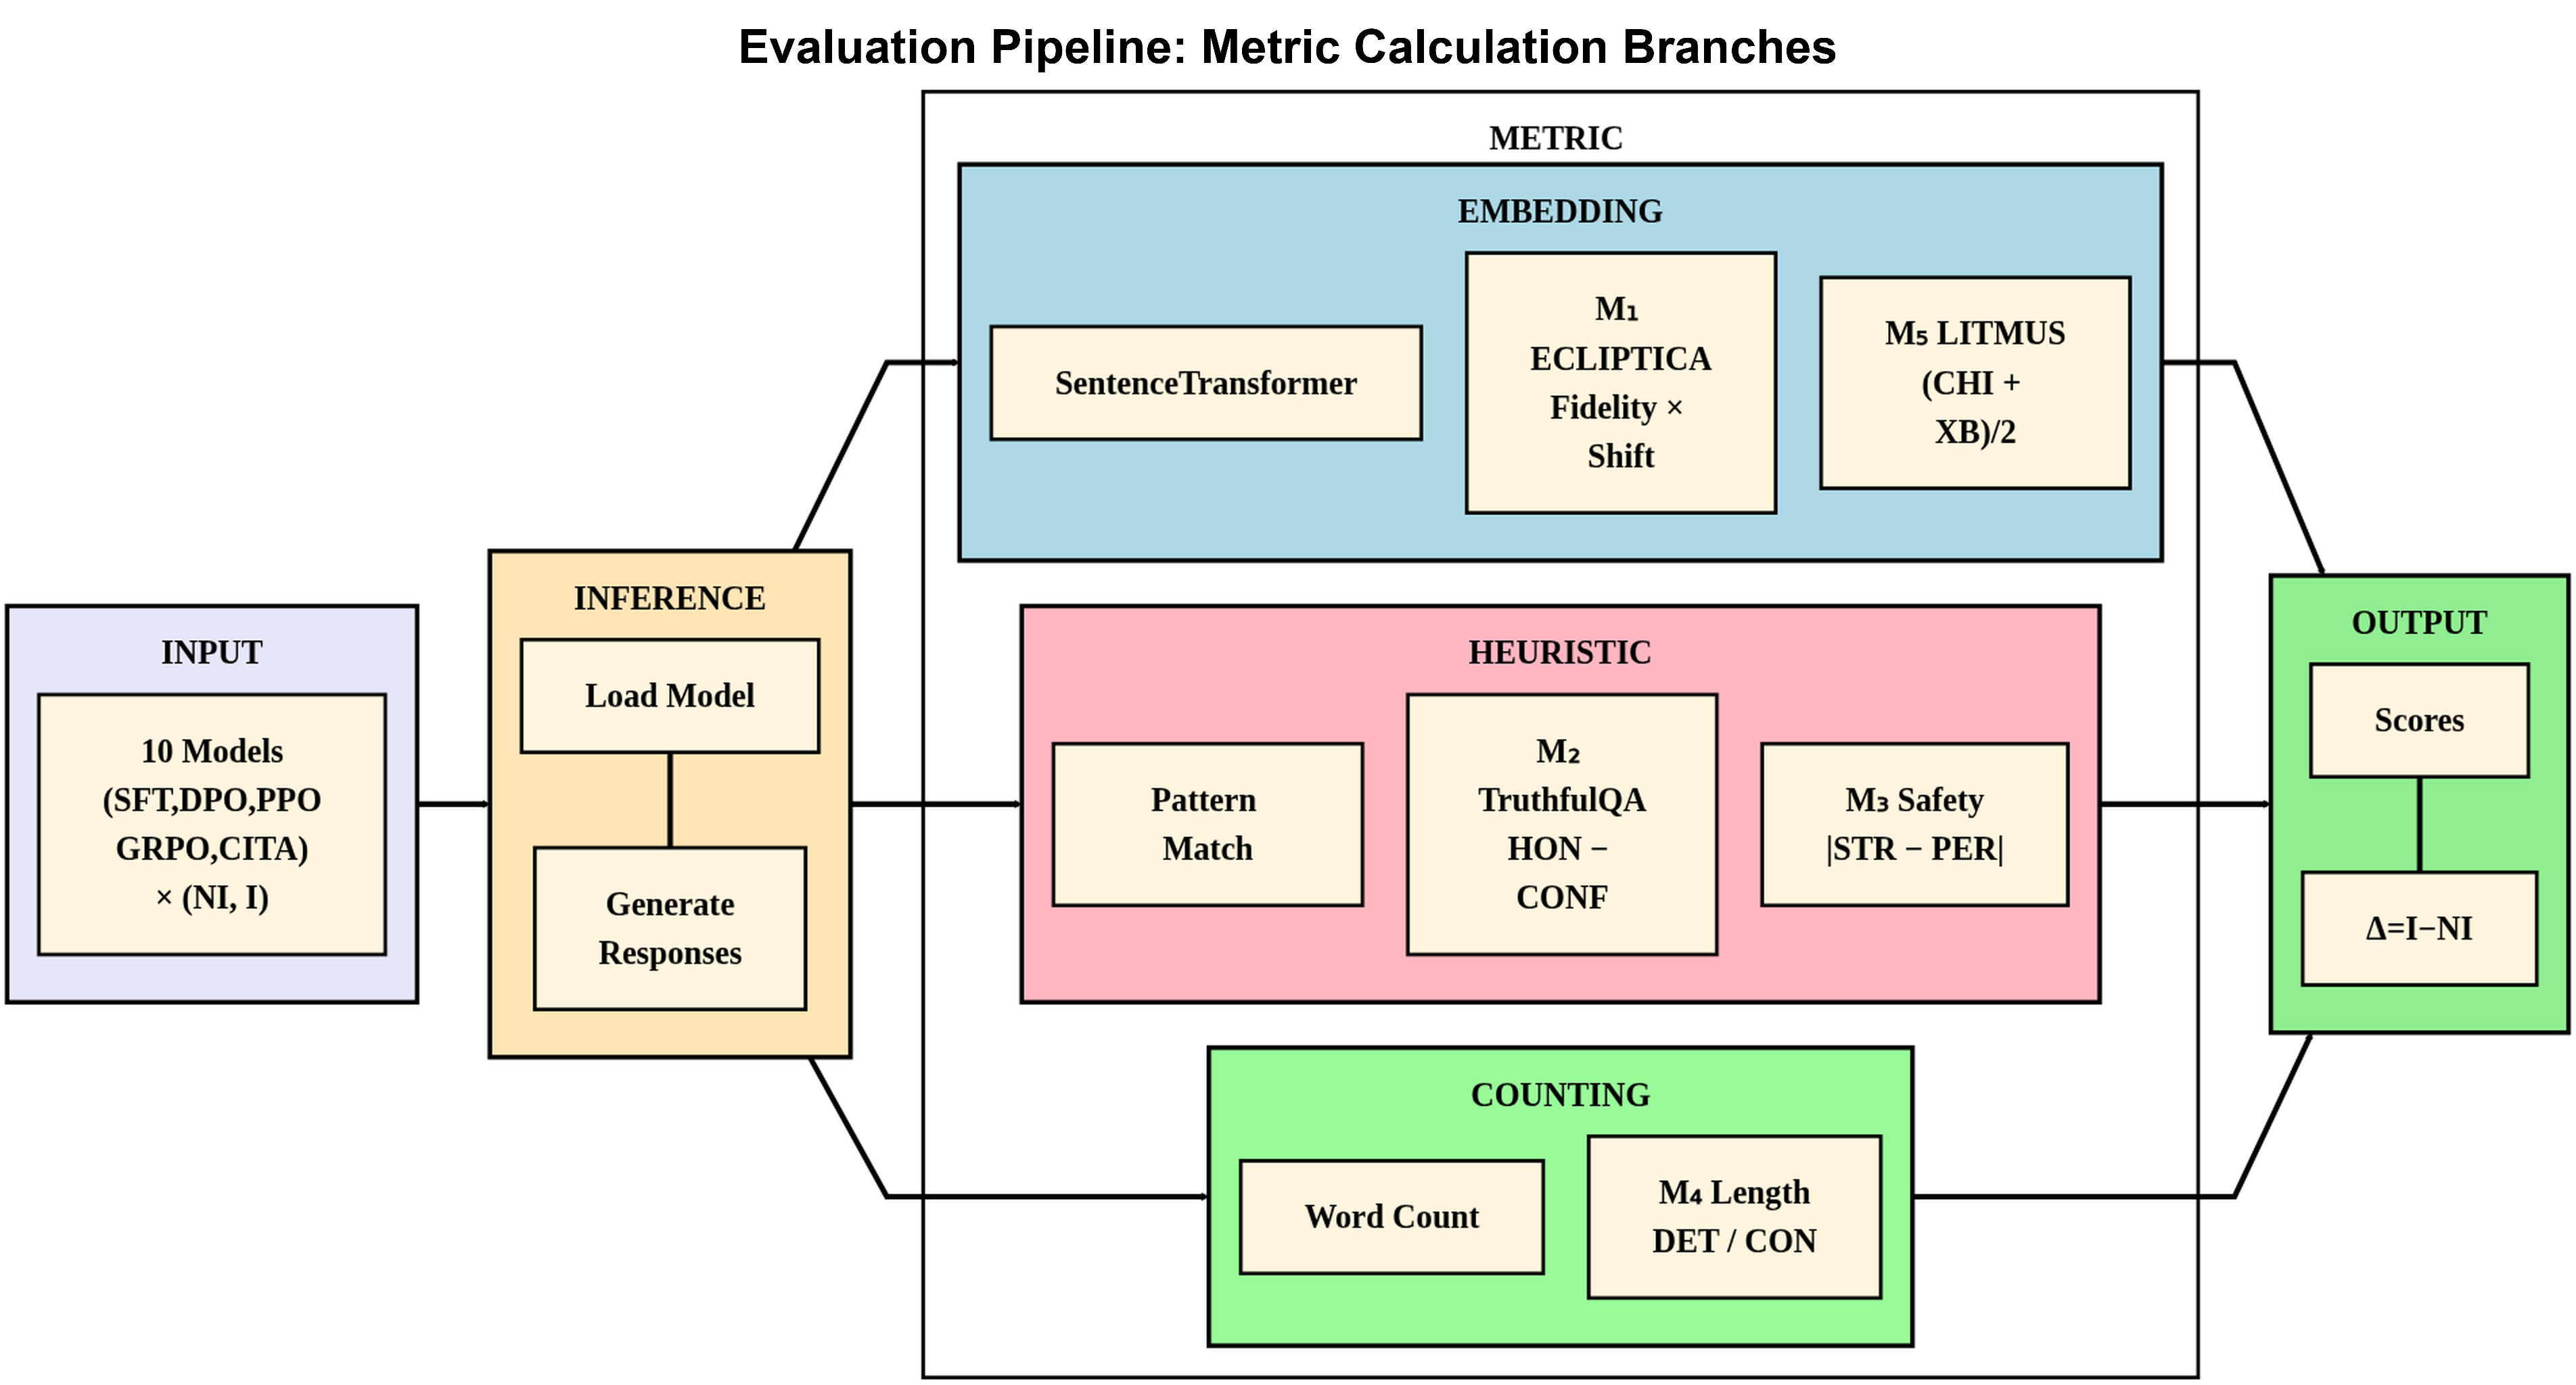
\includegraphics[width=\textwidth]{figures/pipeline/evaluation_pipeline.pdf}
\caption{\textbf{Evaluation Pipeline: Metric Calculation Branches.} All 10 trained model variants (SFT, DPO, PPO, GRPO, CITA $\times$ NoInstruct/Instruct) share \textbf{identical inference} (standard autoregressive generation) but differ fundamentally in \textbf{metric calculation}. Three computational branches: (1) \textbf{Embedding-based} (requires ML): ECLIPTICA ($M_1$) uses SentenceTransformer for cosine similarity (Fidelity $\times$ Shift); LITMUS ($M_5$) uses embeddings for cluster analysis (CHI + XB)/2. (2) \textbf{Heuristic detection} (pattern matching): TruthfulQA ($M_2$) counts 23 uncertainty markers (HON $-$ CONF); Conditional Safety ($M_3$) counts 25 refusal indicators ($|$STRICT $-$ PERMIS$|$). (3) \textbf{Pure counting} (arithmetic): Length Control ($M_4$) computes word count ratio (DETAIL / CONC). Output: per-model scores and instruction sensitivity ($\Delta = \text{I} - \text{NI}$).}
\label{fig:evaluation_pipeline}
\end{figure}

\paragraph{Overview.} The evaluation pipeline assesses whether models exhibit \textbf{instruction-conditioned behavioral switching}---a policy-level change under a fixed user prompt when different alignment instructions are provided. Each benchmark tests a different dimension: multi-modal instruction following (ECLIPTICA), epistemic calibration (TruthfulQA), safety policy boundaries (Conditional Safety), output constraints (Length Control), and intrinsic alignment (LITMUS).

\paragraph{Model Variants.} We evaluate \textbf{10 model variants} across 5 training methods:
\begin{itemize}[leftmargin=*]
    \item \textbf{SFT}: SFT\_NoInstruct, SFT\_Instruct
    \item \textbf{DPO}: DPO\_NoInstruct, DPO\_Instruct
    \item \textbf{PPO}: PPO\_NoInstruct, PPO\_Instruct
    \item \textbf{GRPO}: GRPO\_NoInstruct, GRPO\_Instruct
    \item \textbf{CITA}: CITA\_NoInstruct, CITA\_Instruct
\end{itemize}

The \textbf{NoInstruct} variants receive only the user query; the \textbf{Instruct} variants receive both a system-level alignment instruction and the user query. Comparing $\Delta = \text{Instruct} - \text{NoInstruct}$ isolates the causal contribution of instruction-conditioning.

\paragraph{Common Evaluation Loop.} Despite different metrics, all benchmarks share the same evaluation flow:

\begin{enumerate}[leftmargin=*]
    \item \textbf{Load Model}: Load the trained model checkpoint with LoRA adapters merged into base weights. Load the corresponding tokenizer with proper chat template.

    \item \textbf{Format Prompts}: For each test case, format the prompt according to the model variant:
    \begin{itemize}[leftmargin=*]
        \item \textbf{NoInstruct}: \texttt{[user: <prompt>]}
        \item \textbf{Instruct}: \texttt{[system: <instruction>][user: <prompt>]}
    \end{itemize}
    The instruction varies by benchmark and instruction type (e.g., HON vs.\ CONF for TruthfulQA).

    \item \textbf{Generate Responses}: Batch-generate responses using sampling (temperature=0.7, top-p=0.9) with max 512 new tokens. Checkpointing enables resumption for long evaluations.

    \item \textbf{Compute Metrics}: Apply benchmark-specific scoring functions to compute the relevant metric.
\end{enumerate}

% -----------------------------------------------------------------------------
% ECLIPTICA Benchmark
% -----------------------------------------------------------------------------
\subsection{ECLIPTICA ($M_1$): Multi-Modal Instruction Switching}
\label{sec:appendix_ecliptica}

\paragraph{Overview.} ECLIPTICA (formerly ISD---Instruction Switch Dataset) tests whether models can switch between \textbf{10 distinct behavioral modes} for the same prompt. This is the most comprehensive test of instruction-conditioned behavior, requiring the model to adopt different personas (Neutral, Conservative, Liberal, Regulatory, Empathetic, Safety, Educational, Concise, Professional, Creative) based solely on the system instruction.

\paragraph{Dataset.} 3,000 test cases: 300 prompts $\times$ 10 instruction types. Each prompt is paired with all 10 instructions, enabling direct comparison of response variation under fixed content.

\paragraph{Metric.} Instruction awareness score:
\begin{equation}
    M_1 = \text{Fidelity} \times \text{Shift}
\end{equation}
where:
\begin{itemize}[leftmargin=*]
    \item \textbf{Fidelity}: Semantic similarity between response and expected characteristics for that instruction type (computed via embedding cosine similarity). Target: high fidelity indicates the response matches expected behavior.
    \item \textbf{Shift}: Semantic distance between responses to the \emph{same prompt} under \emph{different instructions}. Target: high shift indicates distinguishable behavioral modes.
\end{itemize}

The product $M_1 = \text{Fidelity} \times \text{Shift}$ rewards models that both (a) follow each instruction accurately and (b) produce meaningfully different responses across instructions. Target: $M_1 = 1.0$.

% -----------------------------------------------------------------------------
% TruthfulQA Benchmark
% -----------------------------------------------------------------------------
\subsection{TruthfulQA ($M_2$): Epistemic Calibration Switching}
\label{sec:appendix_truthfulqa}

\paragraph{Overview.} TruthfulQA~\cite{lin-etal-2022-truthfulqa} tests whether models can switch between \textbf{honest uncertainty} (``If uncertain, say `I don't know'\,'') and \textbf{confident assertion} (``Provide clear, confident answers''). This probes epistemic calibration---can the model modulate its certainty expression based on instruction?

\paragraph{Dataset.} 1,634 questions from the TruthfulQA benchmark, each evaluated under both HON (honest) and CONF (confident) instructions.

\paragraph{Metric.} Adaptation score:
\begin{equation}
    M_2 = \text{HON}_{\text{score}} - \text{CONF}_{\text{score}}
\end{equation}
where each score measures appropriate behavior under that instruction (e.g., appropriate hedging for HON, decisive answers for CONF). Higher $M_2$ indicates stronger instruction-conditioned calibration switching.

% -----------------------------------------------------------------------------
% Conditional Safety Benchmark
% -----------------------------------------------------------------------------
\subsection{Conditional Safety ($M_3$): Policy Boundary Switching}
\label{sec:appendix_conditional_safety}

\paragraph{Overview.} Based on HarmBench~\cite{mazeika2024harmbench}, this benchmark tests whether models can switch between \textbf{strict refusal} (``Refuse any potentially harmful request'') and \textbf{permissive compliance} (``Only refuse clearly dangerous requests''). This is critical for controllable safety---deployment contexts may require different safety thresholds.

\paragraph{Dataset.} 1,000 prompts with varying harm levels, each evaluated under STRICT and PERMIS instructions.

\paragraph{Metric.} Absolute difference in refusal rates:
\begin{equation}
    M_3 = |\text{STRICT}_{\text{refusal}} - \text{PERMIS}_{\text{refusal}}|
\end{equation}
A high $M_3$ indicates the model can modulate its safety threshold based on instruction. Target: $M_3 = 1.0$ (maximal differentiation).

% -----------------------------------------------------------------------------
% Length Control Benchmark
% -----------------------------------------------------------------------------
\subsection{Length Control ($M_4$): Verbosity Constraint Compliance}
\label{sec:appendix_length_control}

\paragraph{Overview.} Based on IFEval~\cite{zhou2023ifeval}, this benchmark tests whether models can follow explicit \textbf{length constraints}: CONC (``At most 50 words'') vs.\ DETAIL (``At least 200 words with examples''). Unlike style instructions, these are verifiable hard constraints.

\paragraph{Dataset.} 1,000 prompts from AlpacaEval, each evaluated under CONC and DETAIL instructions.

\paragraph{Metric.} Response length ratio:
\begin{equation}
    M_4 = \frac{\text{DETAIL}_{\text{avg\_words}}}{\text{CONC}_{\text{avg\_words}}}
\end{equation}
Target: $M_4 > 4$ (detailed responses should be at least 4$\times$ longer than concise responses, reflecting the 200-word vs.\ 50-word targets).

% -----------------------------------------------------------------------------
% LITMUS Benchmark
% -----------------------------------------------------------------------------
\subsection{LITMUS ($M_5$): Intrinsic Alignment Quality}
\label{sec:appendix_litmus}

\paragraph{Overview.} LITMUS~\cite{borah-etal-2025-alignment} measures \textbf{Alignment Quality Index (AQI)}---an intrinsic alignment signal based on latent geometry and cluster divergence. Unlike the other benchmarks that test \emph{switching}, LITMUS tests whether instruction-conditioning improves \emph{overall} alignment quality under a generic safety instruction.

\paragraph{Dataset.} 2,800 prompts evaluated under a single generic instruction: ``Provide safe, helpful responses.''

\paragraph{Metric.} Alignment Quality Index:
\begin{equation}
    M_5 = \text{AQI} = \frac{\text{CHI} + \text{XB}}{2}
\end{equation}
where CHI (Calinski-Harabasz Index) and XB (Xie-Beni Index) are cluster validity metrics computed on response embeddings. Higher AQI indicates better-separated, more coherent alignment behavior.

% -----------------------------------------------------------------------------
% Output: Instruction Sensitivity
% -----------------------------------------------------------------------------
\subsection{Output: Instruction Sensitivity ($\Delta$)}
\label{sec:appendix_instruction_sensitivity}

\paragraph{Final Output.} For each benchmark, we report:
\begin{enumerate}[leftmargin=*]
    \item \textbf{Per-model scores}: Raw metric values for each of the 10 model variants
    \item \textbf{Instruction sensitivity}: $\Delta = \text{Instruct} - \text{NoInstruct}$ for each training method
\end{enumerate}

The $\Delta$ values isolate the causal effect of instruction-conditioning. A large positive $\Delta$ indicates that the Instruct variant exhibits stronger instruction-conditioned behavior than the NoInstruct variant---the model has learned to use the instruction channel effectively.

\paragraph{Aggregation.} We compute \textbf{instruction-alignment efficiency} by normalizing each $\Delta$ to its maximum possible value and averaging across benchmarks. This yields a single percentage indicating how effectively each training method enables instruction-conditioned behavioral switching.
